\documentclass{qqtarticle}

\qqtTitle{TEste 02/02}
\qqtRunningTitle{Automatic Generated Document - Qquant 2022}

\qqtAddAffiliation{1}{Automatic Generated Document}


\qqtAddAuthor{1}{William Kleber}{}

\qqtCorrespondence{\url{http://qquant.online}}
\qqtCorrespondenceEmail{contato@qquant.online}

\qqtAddKeyword{TEste}
\qqtAddKeyword{02/02}
\qqtAddKeyword{teste}

\qqtAbstractPurpose{teste}
\qqtAbstractMethods{teste}
\qqtAbstractResults{<Put your results abstract text here>}
\qqtAbstractConclusion{<Put your conclusion abstract text here>}


\addbibresource{main.bib}

%%%%%%%%%%%%%%%%%%%%%%%%%%%%%%%%%%%%%%%%%%

%---------------------------------------------

% Add latex listing style
\lstdefinestyle{latex}{
   language=[LaTeX]TeX,
    escapeinside={\%*}{*)},
}
\lstdefinelanguage{bibtex}
{keywords={%
@article,@book,@collectedbook,@conference,@electronic,@ieeetranbstctl,%
@inbook,@incollectedbook,@incollection,@injournal,@inproceedings,%
@manual,@mastersthesis,@misc,@patent,@periodical,@phdthesis,@preamble,%
@proceedings,@standard,@string,@techreport,@unpublished%
},
comment=[l][shape]{@comment},
    sensitive=false,
}
\newtheorem*{remark}{Remark} 
\def\biber{\href{https://www.ctan.org/tex-archive/biblio/biber}{\lstinline{biber}}\space}
\def\bibtex{\href{https://www.ctan.org/pkg/bibtex}{\lstinline{bibtex}}\space}

\lstnewenvironment{lstlistingtex}{\lstset{language=[LaTeX]TeX}}{}

% AUTHOR(S): CUSTOM PREAMBLE END
%---------------------------------------------

\begin{document}

% Create the qqt article front page.
\qqtMakeFrontpage

%%%%%%%%%%%%%%%%%%%%%%%%%%%%%%%%%%%%%%%%%%%%%
%%% YOUR ARTICLE BEGINS HERE
%%%%%%%%%%%%%%%%%%%%%%%%%%%%%%%%%%%%%%%%%%%%%

%--------------------------------------------
    \section{General Goals}
    %--------------------------------------------

    <Please use this template to prepare your manuscript for submission to the
    journal for Modeling in Ophthalmology.  You will find here many useful
    instructions on how to organize and format your manuscript.  The main body of
    the manuscript should be contained in a .tex file and the bibliography in a
    .bib file.  The .tex file, the .bib file and the class file should be located in the
    same folder.  For the ease of reference, you are strongly encouraged to name
    the .tex and .bib files as follows: >


    \section{Abstract}
    <Please provide an abstract of 350 words or less. The abstract must be
    structured within the four subheadings above, namely \textit{Purpose},
    \textit{Methods}, \textit{Results} and \textit{Conclusions}. The abstract
    should be informative and appealing to an interdisciplinary audience.>



    \section{PRISMA}
    This diagram was automatically generated.

    \tikzstyle{punktchain} = [rectangle, rounded corners, draw=black, very thick, text width=10em, minimum height=3em, text centered, on chain]

    \tikzstyle{punktfirst} = [ rectangle, rounded corners, draw=black, very thick, text width=10em, minimum height=3em, text centered] % fill=black!10,

    \tikzstyle{punktleft} = [ rectangle, rounded corners, draw=black, text width=7em, minimum height=2em, text centered, fill=blue!8, rotate=90]

    \tikzset{ 
    >=stealth', 
    line/.style={draw, thick, <-}, 
    element/.style={ 
        tape, 
        top color=white, 
        bottom color=blue!50!black!60!, 
        minimum width=8em, 
        draw=blue!40!black!90, very thick, 
        text width=10em,  
        minimum height=3.5em,  
        text centered,  
        on chain}, 
        every join/.style={->, thick,shorten >=1pt}, 
        decoration={brace}, 
        tuborg/.style={decorate}, 
        tubnode/.style={midway, right=2pt} 
    } 

    \begin{figure}[H]
        \begin{center}
            \begin{tikzpicture}
            [node distance=.4cm,
            start chain=going below]
        \node[punktfirst, inner sep=2pt, text width=20mm] (1_db) {PubMed\ (n =  20 )};

        \node[punktfirst, right=of 1_db, inner sep=2pt, text width=20mm] (2_db) {Others\ (n =  0 )};

        \node[punktchain, join,  below=of 1_db] at (3.5,-1) (intro_db) {Records identified through database searching\ (n =  27 )}
        edge[<-]  (1_db)
        edge[<-]  (2_db)
        ;

        \node[punktchain, join] (duplicatas)      {Records after duplicates removed \ (n = 27  )};

        \node[punktchain, join] (screened)      {Records screened \ (n = 19 )};

        \node[punktchain, join] (fulltext)  {Full-text articles assessed for eligibility \ (n = 19 )};

        \node[punktchain, join] (included)      {Studies included in qualitative synthesis \ (n = 19 )};

        \node[punktchain, join] (meta)      {Studies included in quantitative synthesis (meta-analysis) \ (n = 19 )};

        \node[punktfirst, right=of fulltext] (fullexcluded) {Full-text articles excluded, with reasons \ (n =  8 )} edge[<-]  (fulltext);

        \node[punktfirst, right=of screened] (excluded) {Records excluded \ (n = 8 )} edge[<-]  (screened);

        \node[punktleft, text width=30mm]  at (-2.5, -1.5) {Identification};

        \node[punktleft] at (-2.5, -4.7) {Screening};

        \node[punktleft] at (-2.5, -7.8) {Eligibility};

        \node[punktleft] at (-2.5, -11) {Included};

        \end{tikzpicture}
        \end{center}
        \caption{PRISMA Flow Diagram of studies.}
        \label{fig:prisma}
    \end{figure}

    \begin{figure}[H]
        \begin{tikzpicture}[level distance=35mm,node distance=8mm,text height=1.5ex,text depth=0.25ex]
        \begin{scope}[every node/.style={rounded corners,rectangle,thick,minimum width=20mm, minimum height=10mm}]
        \begin{scope}[level 1/.style={sibling distance=19mm,nodes={fill=green!20,draw=green!50}}]
        \node[draw=blue!50,fill=blue!20] (stack) {Qquant Stack} [grow=left]
        child {node (app2) {Protocol}}
        child {node (app1) {Input Data}};
        \end{scope}

        \begin{scope}[level 1/.style={sibling distance=15mm,nodes={fill=yellow!70,draw=yellow!35}}]
        \node[right= of stack,draw=orange!50,fill=orange!20] (ohci) {This Document} [grow=right]
        child {node {Statistics}}
        child {node {Diagrams}}
        child {node {Sections}};
        \end{scope}
        \end{scope}

        \node[below=0mm of app1] (userspace) {User space};
        \node at (userspace -| stack) (kernel) {Processing};
        \node at (userspace -| ohci) (hardware) {Output};

        \path (app1) -- (stack) node[coordinate,midway] (between1) {};
        \draw (ohci) -- (stack) node[coordinate,midway] (between2) {};

        \draw[dashed] (current bounding box.north -| between1) -- (current bounding box.south -| between1);
        \draw[dashed] (current bounding box.north -| between2) -- (current bounding box.south -| between2);
        \end{tikzpicture}
        \caption{This is what We've done with your data.}
        \label{fig:all_steps}
    \end{figure}
    %%%%%%%%%%%%%%%%%%%%%%%%%%%%%%%%%%%%%%%%%%%%%%
    \section{Organization of the Manuscript}

    \subsection{Suggested sections}
    You are strongly encouraged to organize the manuscript into five main sections
    entitled \textit{Introduction}, \textit{Methods}, \textit{Results},
    \textit{Discussions}, \textit{Conclusions and future perspectives}.

    \subsubsection{Introduction}
    Please provide an informative overview of the background motivating your work.
    The introduction of your manuscript is particularly important as it helps
    creating a forum among scientists of different expertise.  Please be sure to
    cite the relevant literature and to clearly identify open questions and/or
    controversial issues in the field.

    \section{Categories and Generated Summaries}
    The following sections are automatically generated categories, all content is for appreciation only, the Qquant group is not responsible for misuse of this information.

    \subsection{<Spelling Observations>}
    <Please set spelling to English-US>.

    \subsection{<Abbreviations Special>}
    <Please use only abbreviations that are common and necessary to the exposition
    of the text. Abbreviations should be widely understood by the qqt
    multi-disciplinary audience that includes ophthalmologists, physiologists,
    mathematicians, engineers and physicists. Introduce each abbreviation in
    parentheses after the first use of the full term. Avoid abbreviations that have
    meaning only within the context of the specific manuscript>.

    \section{Arterial Allografts}
        Results of cryopreserved arterial allograft replacement for thoracic and thoracoabdominal aortic infections.BACKGROUND  Primary and secondary thoracic aortic infections are rare but associated with high morbidity and mortality. There is currently no consensus on their optimal treatment. Arterial allografts have been shown to be resistant to bacterial colonization. Complete excision of infected material, especially synthetic grafts, combined with in situ aortic repair is considered the best treatment of abdominal aortic infections. The aim of this study was to assess the management of thoracic and thoracoabdominal aortic infections using arterial allografts. METHODS  Between January 2009 and December 2017, all patients with thoracic and thoracoabdominal aortic native or graft infections underwent complete excision of infected material and in situ arterial allografting. The end points were the early mortality and morbidity rates and early and late rates of reinfection, graft degeneration, and graft related morbidity. RESULTS  Thirty five patients with a mean age of 65.6 ± 9.2 years were included. Twenty one (60%) cases experienced graft infections and 14 (40%) experienced native aortic infections. Eight (22.8%) patients had visceral fistulas  5 (14.4%) prosthetic esophageal, 1 (2.8%) prosthetic bronchial, 1 (2.8%) prosthetic duodenal, and 1 (2.8%) native aortobronchial. In 12 (34.3%) cases, only the descending thoracic aorta was involved; in 23 (65.7%) cases, the thoracoabdominal aorta was involved. Fifteen (42.8%) patients died during the first month or before discharge  5 of hemorrhage, 4 of multiorgan failure, 3 of ischemic colitis, 2 of pneumonia, and 1 of anastomotic disruption. Eleven (31.5%) patients required early revision surgery  6 (17.1%) for nongraft related hemorrhage, 3 (8.6%) for colectomy, 1 (2.9%) for proximal anastomotic disruption, and 1 (2.9%) for tamponade. One (2.9%) patient who died before discharge experienced paraplegia. One (2.9%) patient experienced stroke. Six (17.1%) patients required postoperative dialysis. Among them, four died before discharge. The mean length of stay in the intensive care unit was 11 ± 10.5 days; the mean length of hospital stay was 32 ± 14 days. During a mean follow up of 32.3 ± 23.7 months, three allograft related complications occurred in survivors (15% of late survivors)  one proximal and one distal false aneurysm with no evidence of reinfection and one allograft enteric fistula. The 1 year and 2 year survival rates were 49.3% and 42.5%, respectively. CONCLUSIONS  Although rare, aortic infections are highly challenging. Surgical management includes complete excision of infected tissues or grafts. Allografts offer a promising solution to aortic graft infection because they appear to resist reinfection; however, the grafts must be observed indefinitely because of the risk of late graft complications.

    \begin{figure}[H]
        \centering
        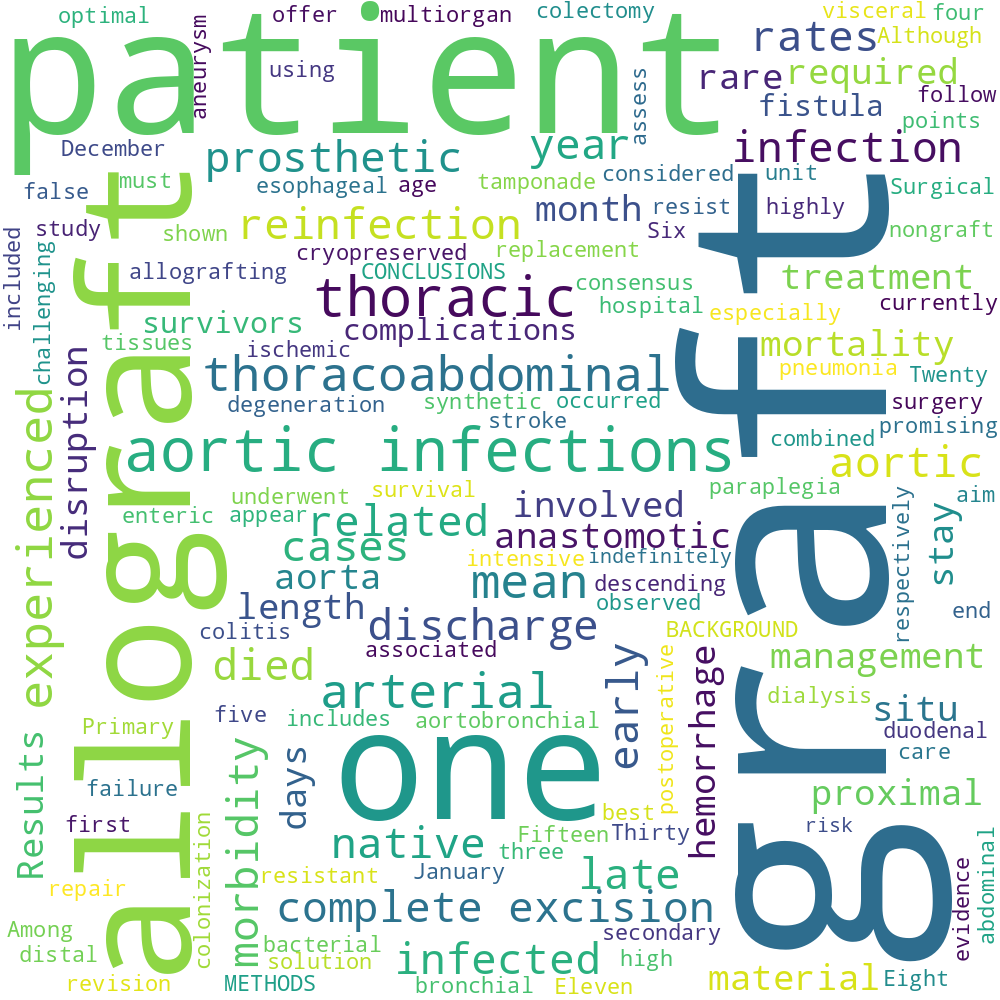
\includegraphics[width=.75\linewidth]{img/arterialallografts.png}
        \caption{Wordcloud of most frequent terms within section arterial allografts.}
        \label{fig:wcl_arterialallografts}
    \end{figure}

    \begin{table}[H]
    \scriptsize
    \centering
    \caption{Articles adherent to section Arterial Allografts}
    \renewcommand{\arraystretch}{1.5}
    \begin{tabular}{p{0.5\textwidth}l}
        \toprule 
        Title & DOI* \\     \midrule Results of cryopreserved arterial allograft replacement for thoracic and thoracoabdominal aortic infections. \cite{Resultsof79533396} & \href{https://dx.doi.org/; 10.1016/j.jvs.2020.05.052}{; 10.1016/j.jvs.2020.05.052}\\     \midrule
        * Clickable item \\
        \bottomrule
    \end{tabular}
    \label{tab:topic1}
    \end{table}\section{Classical Covid 19 Symptoms}
        A case of COVID 19 reinfection in the UK.Protective immunity following COVID 19 infection is not yet fully understood. An understanding of COVID 19 reinfection will be key in guiding government and public health policy decisions in the coming months. This report describes two distinct infective episodes of COVID 19 occurring in the same individual, at the time of writing the first published case in the UK. In April 2020 a 25 year old UK doctor exhibited classical COVID 19 symptoms, including fevers, headaches, and fatigue. A COVID 19 nucleic acid amplification test (NAAT) at the time returned negative. However, a follow up antibody test in May 2020 returned positive. In October 2020 the same individual exhibited coryzal symptoms and headaches. He was COVID 19 NAAT tested and found to be positive. There was exposure to high viral load prior to reinfection. Overall the second infection was symptomatically milder, with a faster recovery. This evidence for reinfection poses challenges for public health and vaccination efforts to protect against the COVID 19 pandemic.

    \begin{figure}[H]
        \centering
        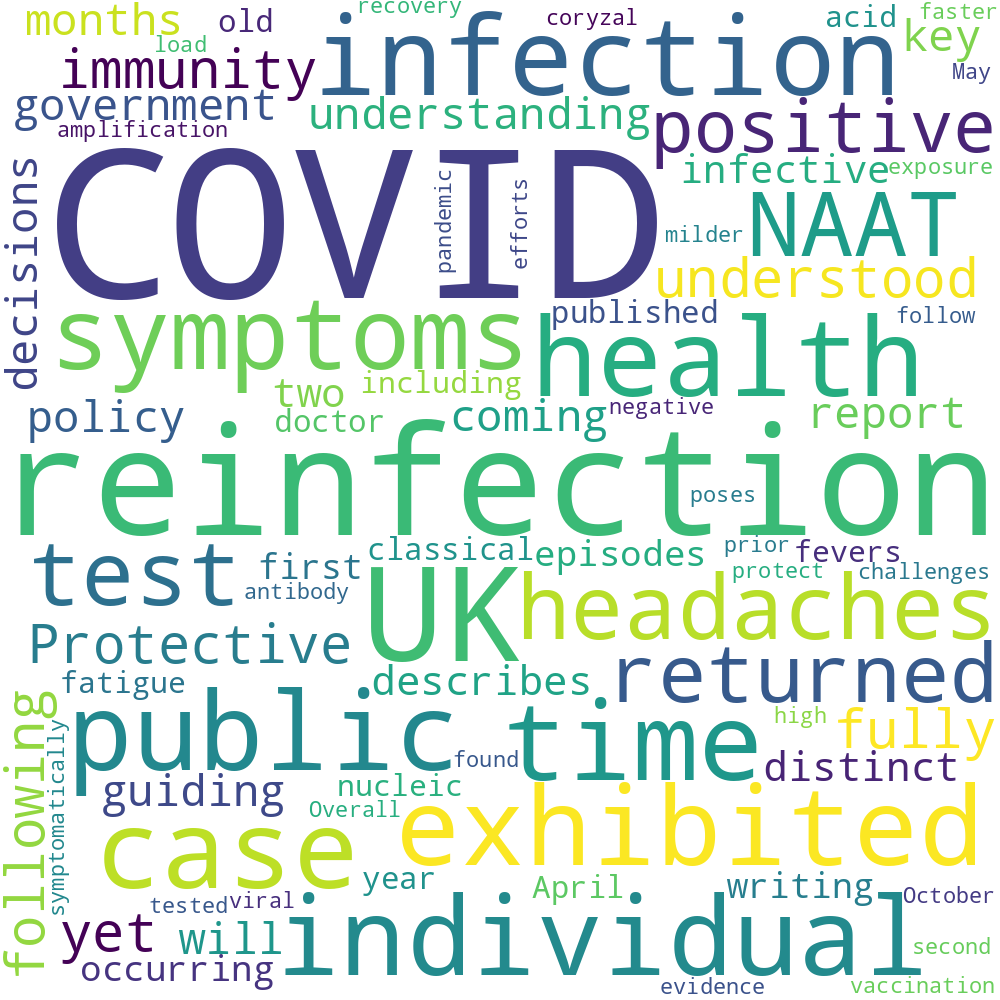
\includegraphics[width=.75\linewidth]{img/classicalcovid19symptoms.png}
        \caption{Wordcloud of most frequent terms within section classical covid 19 symptoms.}
        \label{fig:wcl_classicalcovid19symptoms}
    \end{figure}

    \begin{table}[H]
    \scriptsize
    \centering
    \caption{Articles adherent to section Classical Covid 19 Symptoms}
    \renewcommand{\arraystretch}{1.5}
    \begin{tabular}{p{0.5\textwidth}l}
        \toprule 
        Title & DOI* \\     \midrule A case of COVID 19 reinfection in the UK. \cite{Acaseofd09299c3} & \href{https://dx.doi.org/10.7861/clinmed.2020 0912}{10.7861/clinmed.2020 0912}\\     \midrule
        * Clickable item \\
        \bottomrule
    \end{tabular}
    \label{tab:topic2}
    \end{table}\section{Culture Reinfection}
        Characterization of cerebrospinal fluid (CSF) microbiota from patients with CSF shunt infection and reinfection using high throughput sequencing of 16S ribosomal RNAgenes.BACKGROUND  Nearly 20% of patients with cerebrospinal fluid (CSF) shunt infection develop reinfection. It is unclear whether reinfections are caused by an organism previously present or are independent infection events. OBJECTIVE  We used bacterial culture and high throughput sequencing (HTS) of 16S ribosomal RNA (rRNA) genes to identify bacteria present in serial CSF samples obtained from children who failed CSF shunt infection treatment. We hypothesized that organisms that persist in CSF despite treatment would be detected upon reinfection. DESIGN/METHODS  Serial CSF samples were obtained from 6 patients, 5 with 2 infections and 1 with 3 infections; the study was limited to those for which CSF samples were available from the end of infection and beginning of reinfection. Amplicons of the 16S rRNA gene V4 region were sequenced. Taxonomic assignments of V4 sequences were compared with bacterial species identified in culture. RESULTS  Seven infection dyads averaging 13.5 samples per infection were analyzed. A median of 8 taxa [interquartile range (IQR) 5 10] were observed in the first samples from reinfection using HTS. Conventional culture correlated with high abundance of an organism by HTS in all but 1 infection. In 6 of 7 infection dyads, organisms identified by culture at reinfection were detected by HTS of culture negative samples at the end of the previous infection. The median Chao Jaccard abundance based similarity index for matched infection pairs at end of infection and beginning of reinfection was 0.57 (IQR 0.07 0.87) compared to that for unmatched pairs of 0.40 (IQR 0.10 0.60) [p = 0.46]. CONCLUSION(S)  HTS results were generally consistent with culture based methods in CSF shunt infection and reinfection, and may detect organisms missed by culture at the end of infection treatment but detected by culture at reinfection. However, the CSF microbiota did not correlate more closely within patients at the end of infection and beginning of reinfection than between any two unrelated infections. We cannot reject the hypothesis that sequential infections were independent.

    \begin{figure}[H]
        \centering
        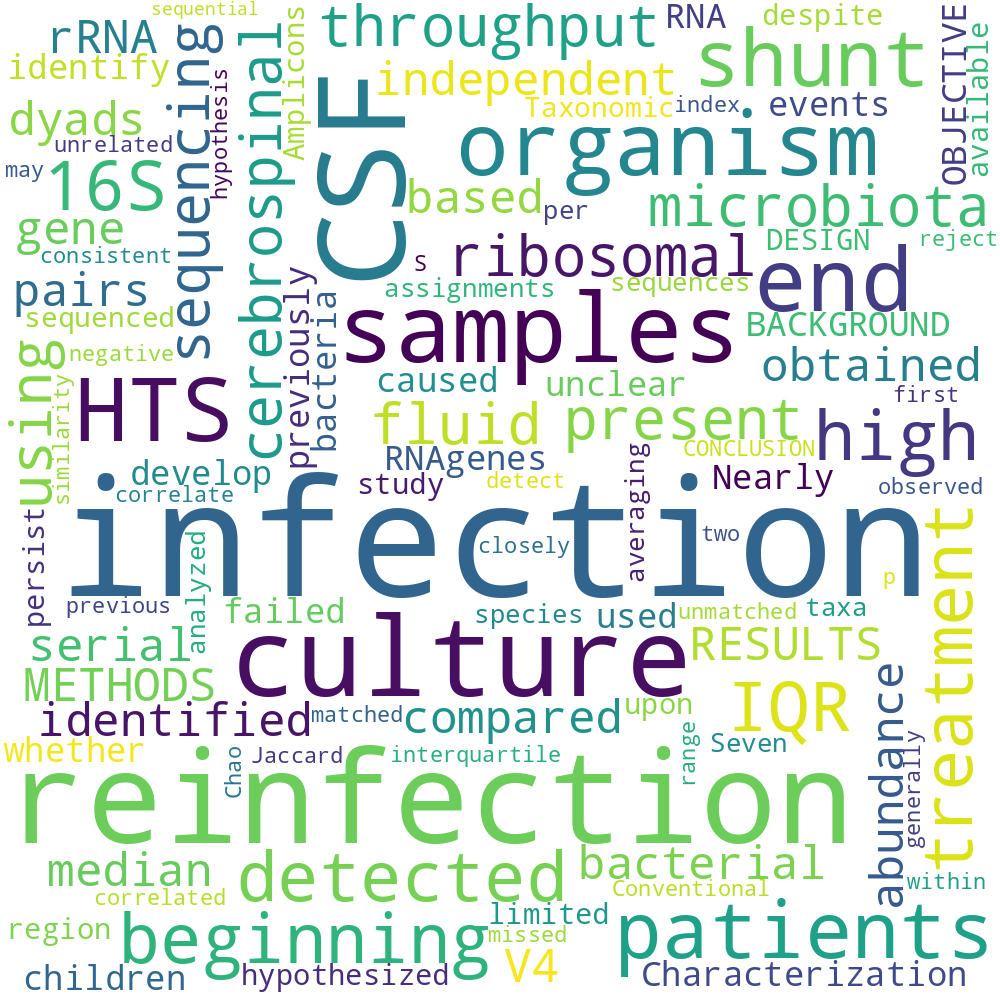
\includegraphics[width=.75\linewidth]{img/culturereinfection.png}
        \caption{Wordcloud of most frequent terms within section culture reinfection.}
        \label{fig:wcl_culturereinfection}
    \end{figure}

    \begin{table}[H]
    \scriptsize
    \centering
    \caption{Articles adherent to section Culture Reinfection}
    \renewcommand{\arraystretch}{1.5}
    \begin{tabular}{p{0.5\textwidth}l}
        \toprule 
        Title & DOI* \\     \midrule Characterization of cerebrospinal fluid (CSF) microbiota from patients with CSF shunt infection and reinfection using high throughput sequencing of 16S ribosomal RNAgenes. \cite{Characterice73373c} & \href{https://dx.doi.org/10.1371/journal.pone.0244643; }{10.1371/journal.pone.0244643; }\\     \midrule
        * Clickable item \\
        \bottomrule
    \end{tabular}
    \label{tab:topic3}
    \end{table}
    
    \section{Direct Acting Antivirals}
        Hepatitis C  clinical management and debated issues.Hepatitis C virus represents an important global health issue with 71 million of infected people in the word. Direct acting antivirals are quite new molecules that hit specific Hepatitis C virus proteins useful for viral replication and assembly. Notably, Direct acting antivirals bring to high sustained virological response rates showing also a great safety profile. This treatment revolution had an impact on transplantation world, in fact the number of liver transplants due to Hepatitis C virus related cirrhosis and hepatocellular carcinoma is quickly decreasing. Even if this therapy has achieved excellent results in terms of morbility and mortality rates' reduction, there are some debated issues to consider. In the present review the main clinical challenges in every day management of Hepatitis C virus patients treated with Direct acting antivirals and the debated effects of viral clearance (metabolic, cardiovascular, immunologic and neoplastic) are discussed. The detection of barriers that can preclude the delivery of Hepatitis C virus care, is the most complex challenge for the scientific community. To obtain the Hepatitis C virus global eradication by 2030, as the World Health Organization has set, will be complex and laborious and will need a further multilevel effort.

    \begin{figure}[H]
        \centering
        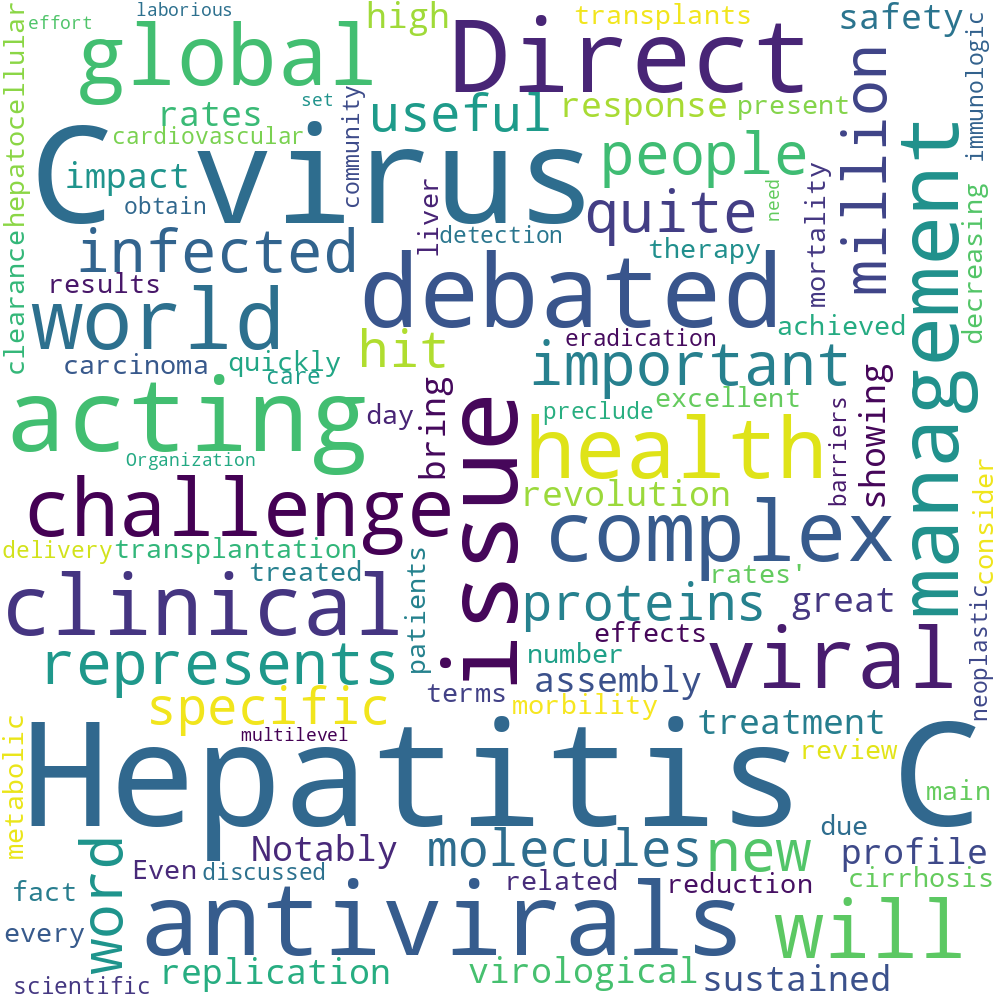
\includegraphics[width=.75\linewidth]{img/directactingantivirals.png}
        \caption{Wordcloud of most frequent terms within section direct acting antivirals.}
        \label{fig:wcl_directactingantivirals}
    \end{figure}

    \begin{table}[H]
    \scriptsize
    \centering
    \caption{Articles adherent to section Direct Acting Antivirals}
    \renewcommand{\arraystretch}{1.5}
    \begin{tabular}{p{0.5\textwidth}l}
        \toprule 
        Title & DOI* \\     \midrule Hepatitis C  clinical management and debated issues. \cite{Hepatitisf57af4b3} & \href{https://dx.doi.org/10.23736/S0026 4806.20.07208 0}{10.23736/S0026 4806.20.07208 0}\\     \midrule
        * Clickable item \\
        \bottomrule
    \end{tabular}
    \label{tab:topic4}
    \end{table}
    
    \section{Ebv Infections}
        Hemophagocytic lymphohistiocytosis secondary to Candida albicans and reactivated EBV 
        infections  A case report and review of the literature.Hemophagocytic lymphohistiocytosis 
        (HLH) has been recognized as a potentially life threatening syndrome. This is the first case 
        of acquired HLH caused by dual infections with Candida albicans and reactivated EBV infections,
         which focuses on the importance of morphological awareness of peripheral blood and bone marrow
          because sometimes they are the only locations that HLH and fungal microorganisms can be 
          diagnosed. A 29 year old woman with a history of abdominal distension and 9 months of 
          intermittent fevers (\$38.8°C) was admitted to the hematology department with treatment for 
          leukopenia and thrombocytopenia. Severe infection of bilateral pulmonary and marked 
          hepatosplenomegaly were detected by computed tomography. EB virus CA IgG, EB virus NA 
          IgG and EB virus CA IgM were positive. Scattered yeast like fungi were found on peripheral 
          blood and bone marrow (BM) smears. BM smears indicated prominent hemophagocytosis. Cultures 
          of bronchoalveolar lavage and BM confirmed the growth of C. albicans. A diagnosis of HLH 
          caused by dual infections with Candida albicans and reactivated EBV infections was 
          established based on the clinical features of the patient because 7 of the 8 diagnostic 
          criteria were met. She was treated with etoposide, dexamethasone for HLH, as well as highly 
          active antifungal and antiviral therapies for the underlying etiology of dual infections. 
          The patient eventually recovered following the effective treatment. 
          A timely and accurate diagnosis is crucial to the prognosis of the dangerous disease.

        \begin{figure}[H]
            \centering
            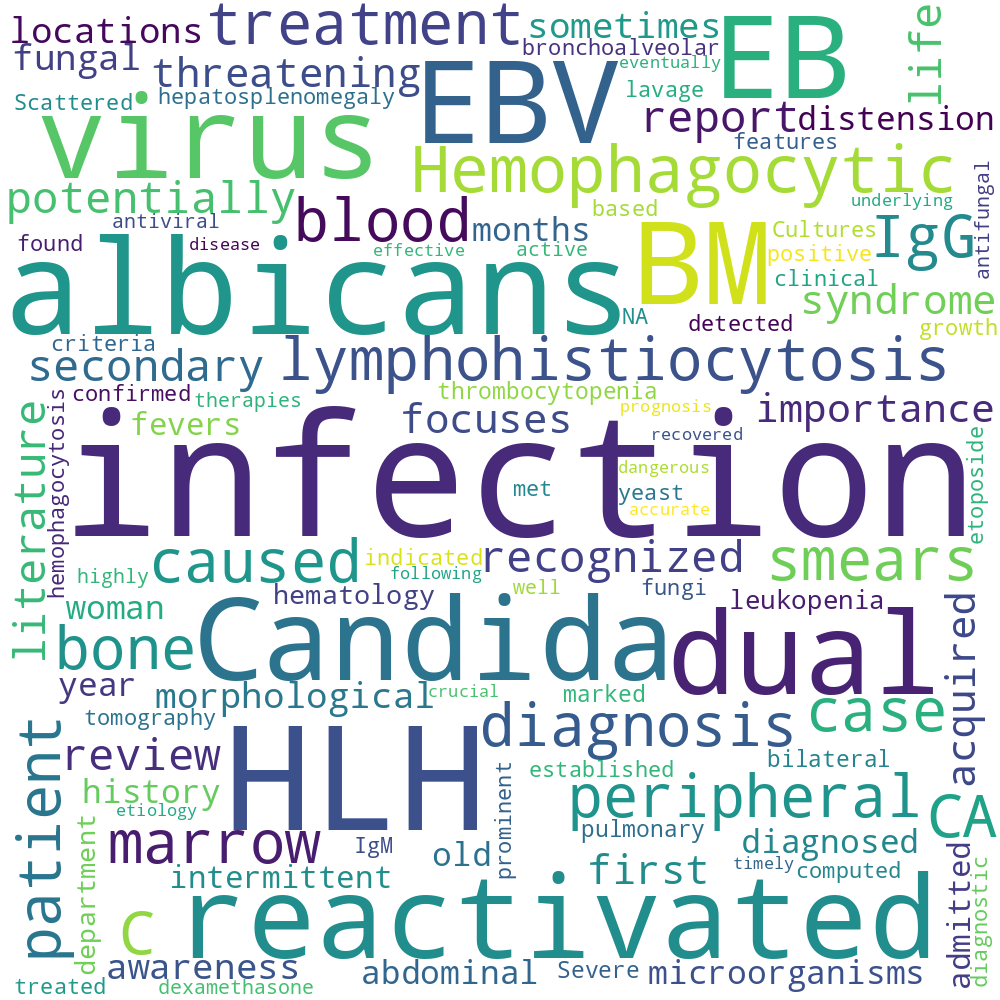
\includegraphics[width=.75\linewidth]{img/ebvinfections.png}
            \caption{Wordcloud of most frequent terms within section ebv infections.}
            \label{fig:wcl_ebvinfections}
        \end{figure}

        \begin{table}[H]
            \scriptsize
            \centering
            \caption{Articles adherent to section Ebv Infections}
            \renewcommand{\arraystretch}{1.5}
            \begin{tabular}{p{0.5\textwidth}l}
                \toprule 
                Title & DOI* \\     \midrule Hemophagocytic lymphohistiocytosis secondary to Candida albicans and reactivated EBV infections  A case report and review of the literature. \cite{Hemophagoc4bb4a422} & \href{https://dx.doi.org/10.4103/IJPM.IJPM_457_20}{10.4103/IJPM.IJPM_457_20}\\     \midrule
                * Clickable item \\
                \bottomrule
            \end{tabular}
            \label{tab:topic5}
        \end{table}
    
    \section{Gastrointestinal Diseases}
        Characteristics of late recurrent candidemia in adult patients.BACKGROUND AND OBJECTIVES  Candida species are one of the most common causes of health care associated bloodstream infections. However, recurrent candidemia is rare, and the characteristics of late recurrent (LR) candidemia are partly unclear. Our aim was to evaluate the characteristics of LR candidemia in adult patients. PATIENTS AND METHODS  A retrospective cohort study was performed in the hospital district of Helsinki and Uusimaa in Finland (2007 2016). All candidemia cases were searched in an electronic database during the study period. Patients with LR candidemia were compared with patients with a single candidemia episode to evaluate the characteristics of LR candidemia. LR candidemia was defined as having at least two episodes of candidemia more than 30 days apart. RESULTS  We identified 24 episodes of LR candidemia in 20 patients. Patients with LR candidemia represented 6% of all patients with candidemia during the study period, and most of these cases were nosocomial. The median time between the first and the recurrent episode was 5.1 months. One year mortality in LR candidemia was 45%. Underlying gastrointestinal disease (OR 7.21, 95% CI 2.52 20.61) and history of intra venous drug use (IVDU) (OR 3.62, 95% CI 1.03 12.69) were independent risk factors for LR candidemia in the multivariable analysis. CONCLUSION  Our study indicates that the gastrointestinal tract may be a continuous source of infection in patients with chronic gastrointestinal diseases. Gastrointestinal diseases and IVDU should be regarded as risk factors for LR candidemia.

        \begin{figure}[H]
            \centering
            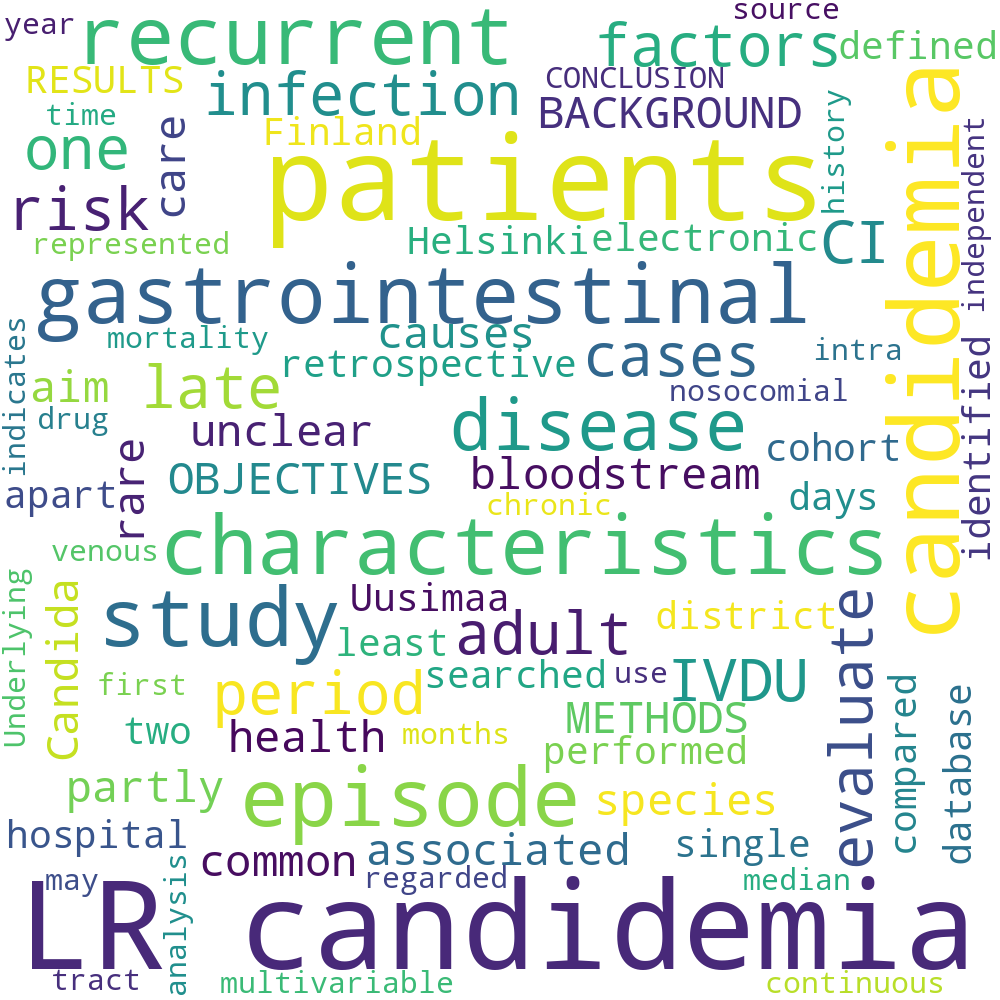
\includegraphics[width=.75\linewidth]{img/gastrointestinaldiseases.png}
            \caption{Wordcloud of most frequent terms within section gastrointestinal diseases.}
            \label{fig:wcl_gastrointestinaldiseases}
        \end{figure}

        \begin{table}[H]
            \scriptsize
            \centering
            \caption{Articles adherent to section Gastrointestinal Diseases}
            \renewcommand{\arraystretch}{1.5}
            \begin{tabular}{p{0.5\textwidth}l}
                \toprule 
                Title & DOI* \\     \midrule Characteristics of late recurrent candidemia in adult patients. \cite{Characteri6287ec6b} & \href{https://dx.doi.org/10.1111/myc.13236}{10.1111/myc.13236}\\     \midrule
                * Clickable item \\
                \bottomrule
            \end{tabular}
            \label{tab:topic6}
        \end{table}
        
    \section{Infectious Disease Epidemiology}
        Responsible modelling  Unit testing for infectious disease epidemiology.Infectious disease epidemiology is increasingly reliant on large scale computation and inference. Models have guided health policy for epidemics including COVID 19 and Ebola and endemic diseases including malaria and tuberculosis. Yet a coding bug may bias results, yielding incorrect conclusions and actions causing avoidable harm. We are ethically obliged to make our code as free of error as possible. Unit testing is a coding method to avoid such bugs, but it is rarely used in epidemiology. We demonstrate how unit testing can handle the particular quirks of infectious disease models and aim to increase the uptake of this methodology in our field.

        \begin{figure}[H]
            \centering
            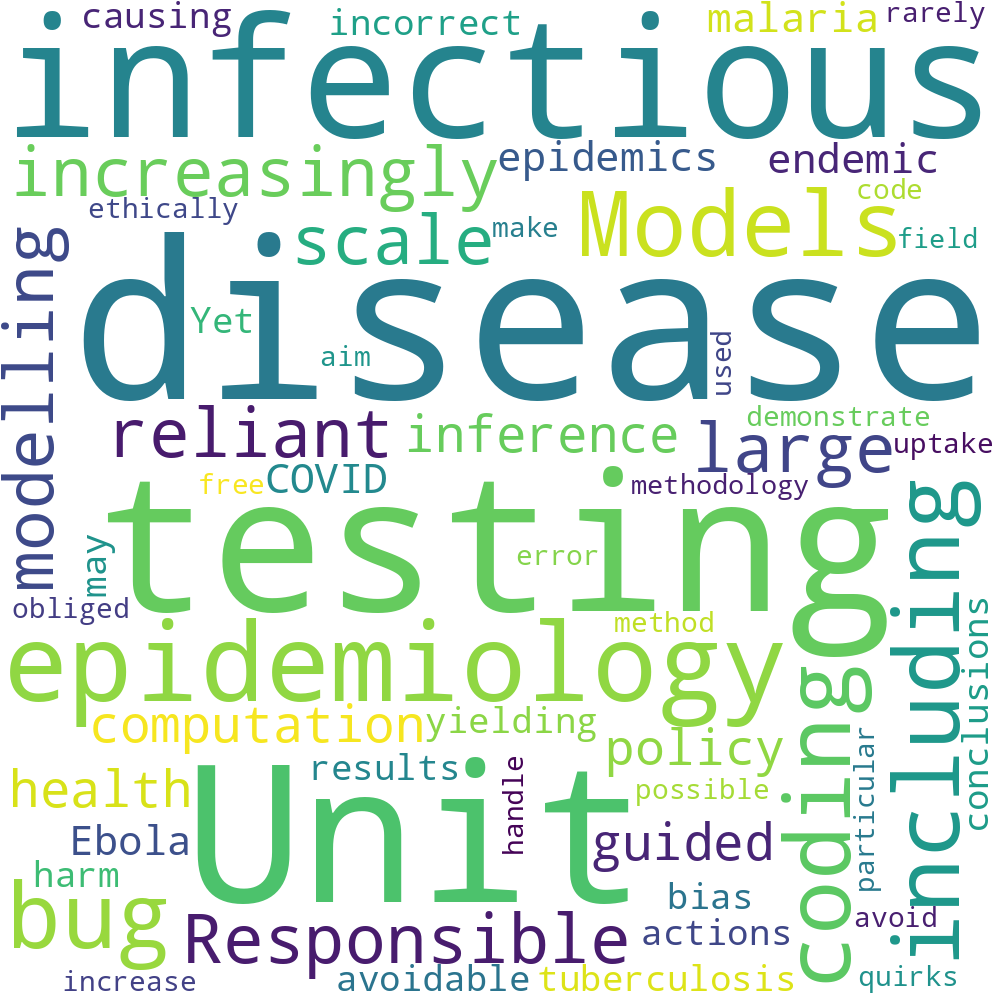
\includegraphics[width=.75\linewidth]{img/infectiousdiseaseepidemiology.png}
            \caption{Wordcloud of most frequent terms within section infectious disease epidemiology.}
            \label{fig:wcl_infectiousdiseaseepidemiology}
        \end{figure}

        \begin{table}[H]
        \scriptsize
        \centering
        \caption{Articles adherent to section Infectious Disease Epidemiology}
        \renewcommand{\arraystretch}{1.5}
        \begin{tabular}{p{0.5\textwidth}l}
            \toprule 
            Title & DOI* \\     \midrule Responsible modelling  Unit testing for infectious disease epidemiology. \cite{Responsibl7050b63e} & \href{https://dx.doi.org/; 10.1016/j.epidem.2020.100425; }{; 10.1016/j.epidem.2020.100425; }\\     \midrule
            * Clickable item \\
            \bottomrule
        \end{tabular}
        \label{tab:topic7}
        \end{table}\section{P. Yoelii}
            Immune characteristics of Plasmodium reinfections in mice following chloroquine cure of primary Plasmodium infections.OBJECTIVE  To investigate the disease progression and immunoprotective characteristics in mice re infected with homogeneous/heterogeneous Plasmodium strains following cure of Plasmodium infections with chloroquine at the peak of parasitemia. METHODS  C57BL/6 mice were infected with the non lethal P. yoelii 17XNL strain, and half of mice were given treatment with chloroquine at the peak of parasitemia (9 days post infection), while the other mice were self cured naturally. Then, all cured mice were re infected with the equivalent lethal P. yoelii 17XL or P. berghei ANKA strain 90 days following primary Plasmodium infections. The parasitemia levels during primary infections and reinfections were measured by microscopic examinations of Giemsa stained thin blood films, and the levels of the IgG antibody in sera and the percentages of memory T cell subsets in spleen cells were detected in mice using ELISA and flow cytometry before and after parasite reinfections, respectively. RESULTS  Following primary infections with the P. yoelii 17XNL strain, the serum IgG antibody levels were (5.047 ± 0.924) pg/mL in the selfcured mice and (4.429 ± 0.624) pg/mL in the chloroquine treated mice, respectively (t = 0.437, P > 0.05), which were both significantly higher than that in the uninfected mice (1.624 pg/mL ± 0.280 pg/mL) (F = 22.522, P < 0.01). There was no significant difference in the serum IgG antibody level among self cured and chloroquine treated mice re infected with the P. yoelii 17XL strain or the P. berghei ANKA strain (F = 0.542, P > 0.05); however, the serum IgG antibody levels were all significantly higher in selfcured and chloroquine treated mice re infected with the P. yoelii 17XLstrain[(15.487±1.173)pg/mLand(15.965±1.150)pg/mL] or the P. berghei ANKA strain [(14.644 ± 1.523) pg/mL and (15.185 ± 1.333) pg/mL] relative to primary infections (F = 67.383, P < 0.01). There was no significant difference in the proportion of CD4(+) [(34.208 ± 2.106), (32.820 ± 1.930), (34.023 ± 2.289), (35.608 ± 1.779) pg/mL] or CD8(+) T memory cells [(17.935 ± 2.092), (18.918 ± 2.823), (17.103 ± 1.627), (17.873 ± 1.425) pg/mL] in self cured and chloroquine treated mice with primary infections with the P. yoelii 17XNL strain followed by re infections with the P. yoelii 17XL strain or the P. berghei ANKA strain (F = 0.944 and 0.390, both P > 0.05); however, the proportions of the CD4(+) or CD8(+) T memory cells were significantly greater in self cured and chloroquine treated mice with primary infections with the P. yoelii 17XNL strain followed by re infections with the P. yoelii 17XL strain or the P. berghei ANKA strain than in mice with primary infections (F = 50.532 and 21.751, both P < 0.01). CONCLUSIONS  The cure of murine Plasmodium infections with chloroquine does not affect the production of effective immune protections in mice during parasite re infections. Following a primary infection, mice show a protection against re infections with either homogeneous or heterogeneous Plasmodium strains, and a higher level resistance to re infections with homogeneous parasite strains is found than with heterogeneous strains.

        \begin{figure}[H]
            \centering
            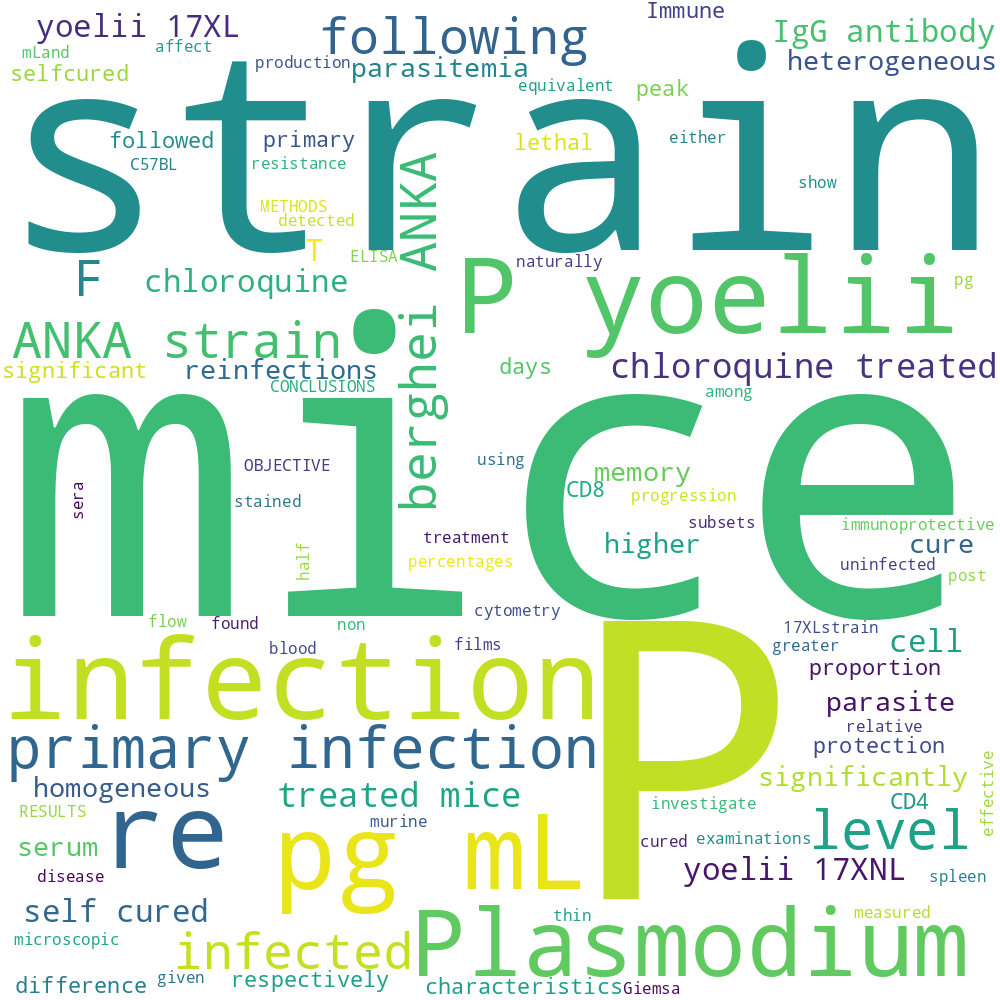
\includegraphics[width=.75\linewidth]{img/p.yoelii.png}
            \caption{Wordcloud of most frequent terms within section p. yoelii.}
            \label{fig:wcl_p.yoelii}
        \end{figure}

        \begin{table}[H]
        \scriptsize
        \centering
        \caption{Articles adherent to section P. Yoelii}
        \renewcommand{\arraystretch}{1.5}
        \begin{tabular}{p{0.5\textwidth}l}
            \toprule 
            Title & DOI* \\     \midrule Immune characteristics of Plasmodium reinfections in mice following chloroquine cure of primary Plasmodium infections. \cite{Immunechae26fb43e} & \href{https://dx.doi.org/10.16250/j.32.1374.2020164}{10.16250/j.32.1374.2020164}\\     \midrule
            * Clickable item \\
            \bottomrule
        \end{tabular}
        \label{tab:topic8}
        \end{table}\section{Prior Sars Cov 2 Infection}
            Prior SARS CoV 2 infection is associated with protection against symptomatic reinfection.• Whether SARS CoV 2 infection confers immunity to reinfection is uncertain. • The ‘second wave’ of transmission offered an opportunity to examine this. • We observed no symptomatic reinfections in a cohort of healthcare workers. • This apparent immunity to re infection was maintained for at least 6 months. • Further studies are required to define immunological mechanism(s) and durability.

        \begin{figure}[H]
            \centering
            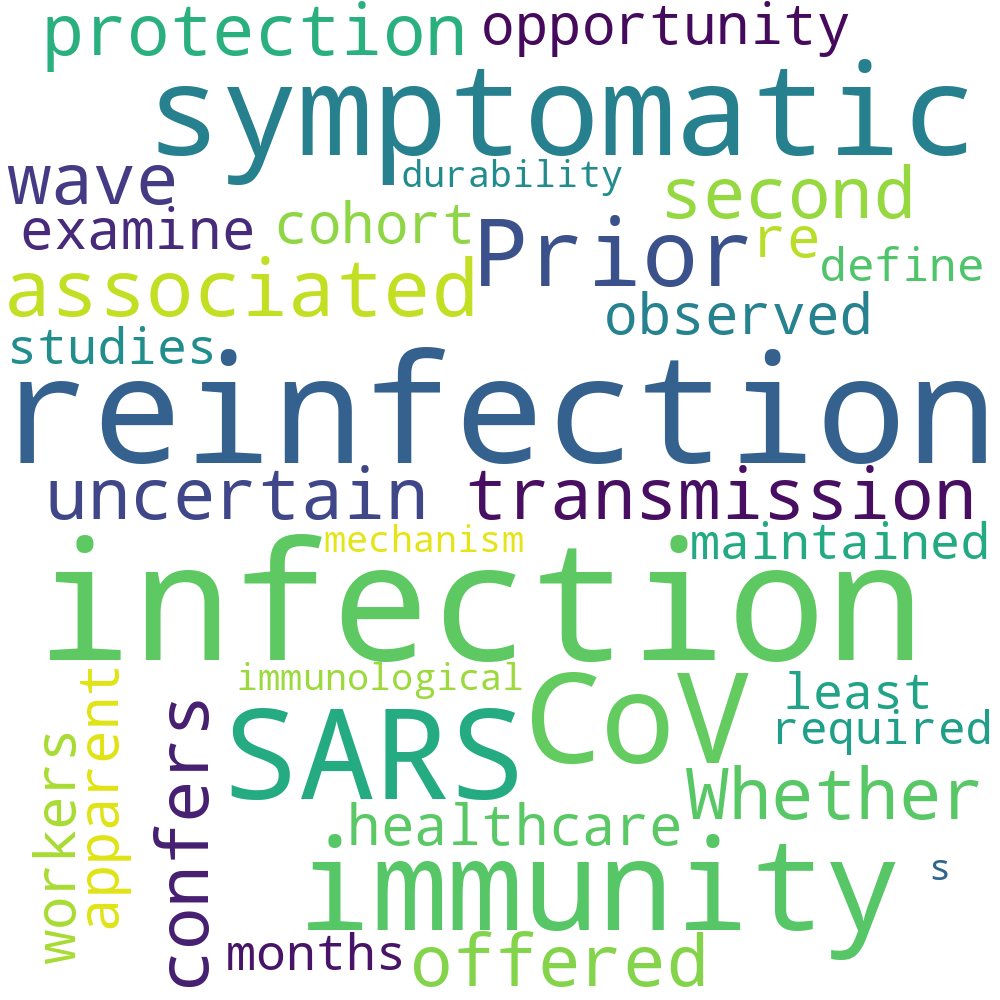
\includegraphics[width=.75\linewidth]{img/priorsarscov2infection.png}
            \caption{Wordcloud of most frequent terms within section prior sars cov 2 infection.}
            \label{fig:wcl_priorsarscov2infection}
        \end{figure}

        \begin{table}[H]
        \scriptsize
        \centering
        \caption{Articles adherent to section Prior Sars Cov 2 Infection}
        \renewcommand{\arraystretch}{1.5}
        \begin{tabular}{p{0.5\textwidth}l}
            \toprule 
            Title & DOI* \\     \midrule Prior SARS CoV 2 infection is associated with protection against symptomatic reinfection. \cite{PriorSARSd192fef2} & \href{https://dx.doi.org/; 10.1016/j.jinf.2020.12.023}{; 10.1016/j.jinf.2020.12.023}\\     \midrule
            * Clickable item \\
            \bottomrule
        \end{tabular}
        \label{tab:topic9}
        \end{table}\section{Recommendations Patients}
            Symptomatic relapse and long term sequelae of COVID 19 in a previously healthy 30 year old man.Much has been reported on the clinical course of severe COVID 19, but less is known about the natural history and sequalae of mildly symptomatic cases and the prospects of reinfection or recurrence of symptoms. We report a case of a patient with mildly symptomatic PCR confirmed COVID 19 who, after being symptom free for 2 weeks, redeveloped symptoms and was found to be PCR positive again >4 weeks from original testing. Surprisingly, IgG and IgM antibody testing was negative 2 months after reinfection. Although no negative testing was performed between the two symptomatic bouts, this case raises the possibility of reinfection after controlling the virus and highlights the long period with which a patient can shed virus and experience symptoms after initial infection. Characterising variations in clinical symptoms and length of viral shedding after improvement is essential for informing recommendations on patients safely resuming contact with others.

        \begin{figure}[H]
            \centering
            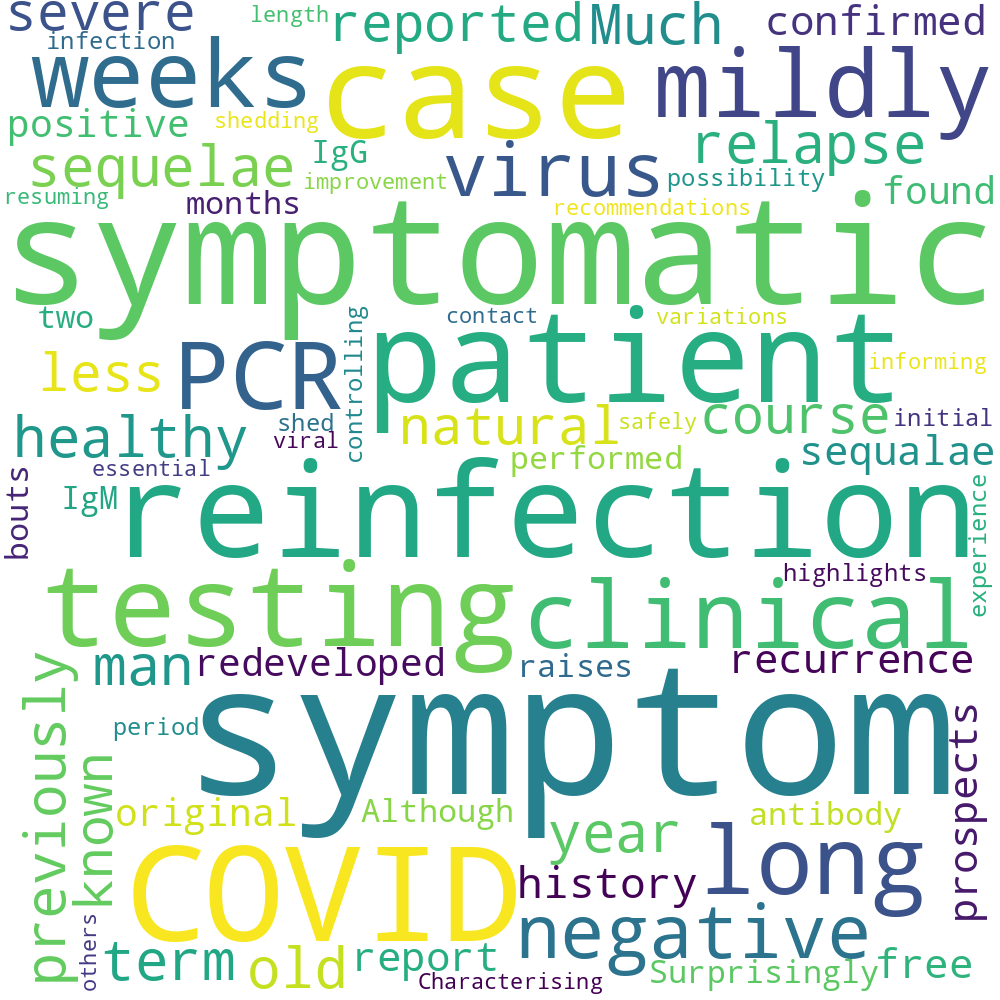
\includegraphics[width=.75\linewidth]{img/recommendationspatients.png}
            \caption{Wordcloud of most frequent terms within section recommendations patients.}
            \label{fig:wcl_recommendationspatients}
        \end{figure}

        \begin{table}[H]
        \scriptsize
        \centering
        \caption{Articles adherent to section Recommendations Patients}
        \renewcommand{\arraystretch}{1.5}
        \begin{tabular}{p{0.5\textwidth}l}
            \toprule 
            Title & DOI* \\     \midrule Symptomatic relapse and long term sequelae of COVID 19 in a previously healthy 30 year old man. \cite{Symptomati7b5ae66e} & \href{https://dx.doi.org/10.1136/bcr 2020 239825; }{10.1136/bcr 2020 239825; }\\     \midrule
            * Clickable item \\
            \bottomrule
        \end{tabular}
        \label{tab:topic10}
        \end{table}\section{Sars Cov}
            SARS CoV 2 reinfection and implications for vaccine development.Coronavirus disease 2019 (COVID 19) pandemic continues to constitute a public health emergency of international concern. Multiple vaccine candidates for COVID 19, which is caused by severe acute respiratory syndrome coronavirus 2 (SARS CoV 2), have entered clinical trials. However, some evidence suggests that patients who have recovered from COVID 19 can be reinfected. For example, in China, two discharged COVID 19 patients who had recovered and fulfilled the discharge criteria for COVID 19 were retested positive to a reverse transcription polymerase chain reaction (RT PCR) assay for the virus. This finding is critical and could hamper COVID 19 vaccine development. This review offers literature based evidence of reinfection with SARS CoV 2, provides explanation for the possibility of SARS CoV 2 reinfection both from the agent and host points of view, and discusses its implication for COVID 19 vaccine development.Antibody response and therapy in COVID 19 patients  what can be learned for vaccine development The newly emerged severe acute respiratory syndrome coronavirus 2 (SARS CoV 2) has infected millions of people and caused tremendous morbidity and mortality worldwide. Effective treatment for coronavirus disease 2019 (COVID 19) due to SARS CoV 2 infection is lacking, and different therapeutic strategies are under testing. Host humoral and cellular immunity to SARS CoV 2 infection is a critical determinant for patients' outcomes. SARS CoV 2 infection results in seroconversion and production of anti SARS CoV 2 antibodies. The antibodies may suppress viral replication through neutralization but might also participate in COVID 19 pathogenesis through a process termed antibody dependent enhancement. Rapid progress has been made in the research of antibody response and therapy in COVID 19 patients, including characterization of the clinical features of antibody responses in different populations infected by SARS CoV 2, treatment of COVID 19 patients with convalescent plasma and intravenous immunoglobin products, isolation and characterization of a large panel of monoclonal neutralizing antibodies and early clinical testing, as well as clinical results from several COVID 19 vaccine candidates. In this review, we summarize the recent progress and discuss the implications of these findings in vaccine development.Covid 19 reinfections  what is the clinical relevance .Every day additional confirmed case of SARS CoV 2 reinfection are being reported across the globe. In the Netherlands more than 50 cases of probable reinfections have been identified. With more than 500 thousand people in the Netherlands who have been infected with SARS CoV 2 up till now this number does seems to be quite low. Still, important questions have to be asked. How do we define reinfection and how do these reinfections compare to other (corona) viruses  What is the immunological significance  What is the duration of protective immunity  And what does Covid 19 reinfections mean for the prevention and development of a vaccine  The described cases of re infections do teach us that a SARS CoV 2 vaccine should also be considered for people with a documented Covid 19 infection in the past and that general precautions, such as the use of face masks and social distancing, still apply to those with a previous SARS CoV 2 infection.Immunological characteristics govern the transition of COVID 19 to endemicity.We are currently faced with the question of how the severity of infection with severe acute respiratory syndrome coronavirus 2 (SARS CoV 2) may change in the years ahead. Our analysis of immunological and epidemiological data on endemic human coronaviruses (HCoVs) shows that infection blocking immunity wanes rapidly but that disease reducing immunity is long lived. Our model, incorporating these components of immunity, recapitulates both the current severity of SARS CoV 2 infection and the benign nature of HCoVs, suggesting that once the endemic phase is reached and primary exposure is in childhood, SARS CoV 2 may be no more virulent than the common cold. We predict a different outcome for an emergent coronavirus that causes severe disease in children. These results reinforce the importance of behavioral containment during pandemic vaccine rollout, while prompting us to evaluate scenarios for continuing vaccination in the endemic phase.Understanding the outcomes of COVID 19   does the current model of an acute respiratory infection really fit Although coronavirus disease 2019 (COVID 19) is regarded as an acute, resolving infection followed by the development of protective immunity, recent systematic literature review documents evidence for often highly prolonged shedding of severe acute respiratory syndrome coronavirus 2 (SARS CoV 2) in respiratory and faecal samples, periodic recurrence of PCR positivity in a substantial proportion of individuals and increasingly documented instances of reinfection associated with a lack of protective immunity. This pattern of infection is quite distinct from the acute/resolving nature of other human pathogenic respiratory viruses, such as influenza A virus and respiratory syncytial virus. Prolonged shedding of SARS CoV 2 furthermore occurs irrespective of disease severity or development of virus neutralizing antibodies. SARS CoV 2 possesses an intensely structured RNA genome, an attribute shared with other human and veterinary coronaviruses and with other mammalian RNA viruses such as hepatitis C virus. These are capable of long term persistence, possibly through poorly understood RNA structure mediated effects on innate and adaptive host immune responses. The assumption that resolution of COVID 19 and the appearance of anti SARS CoV 2 IgG antibodies represents virus clearance and protection from reinfection, implicit for example in the susceptible infected recovered (SIR) model used for epidemic prediction, should be rigorously re evaluated.Coronavirus disease 2019 (COVID 19) pandemic continues to constitute a public health emergency of international concern. Multiple vaccine candidates for COVID 19, which is caused by severe acute respiratory syndrome coronavirus 2 (SARS CoV 2), have entered clinical trials. Some evidence suggests that patients who have recovered from CO VID 19 can be reinfected. This finding is critical and could hamper vaccine development.

        \begin{figure}[H]
            \centering
            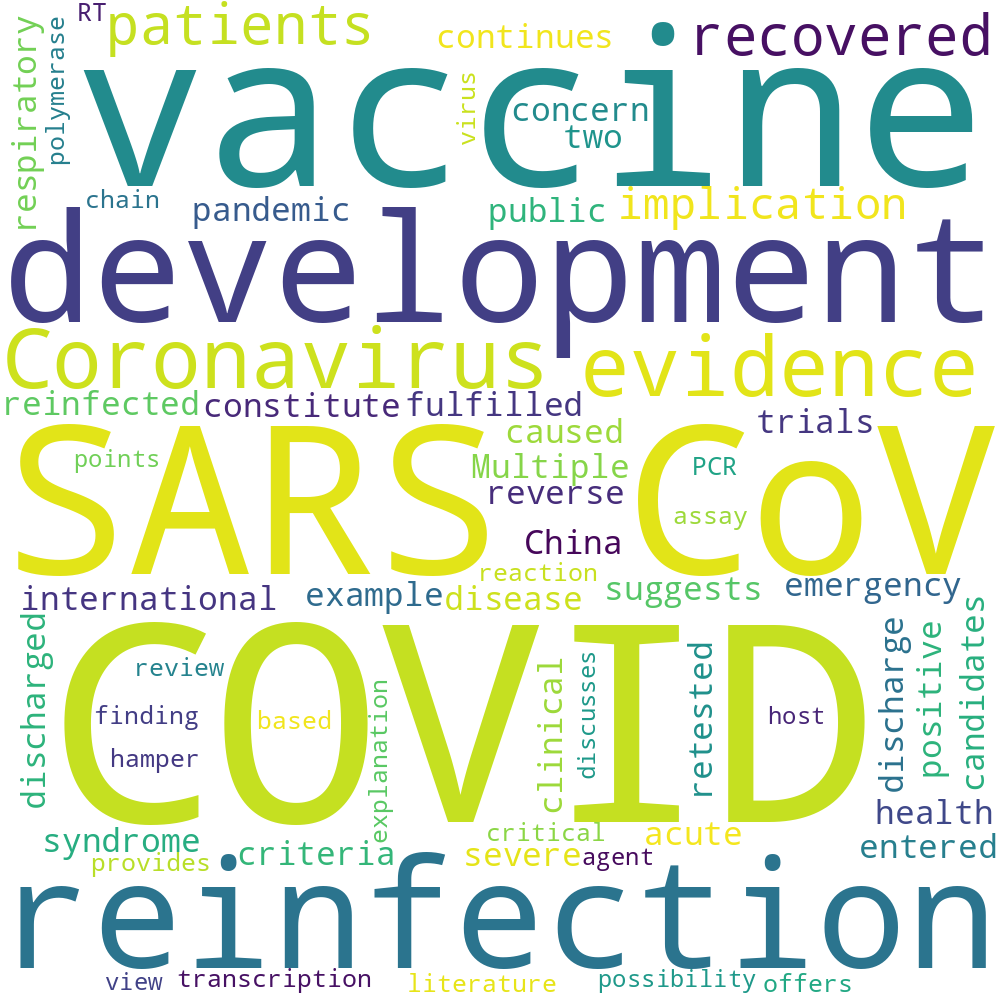
\includegraphics[width=.75\linewidth]{img/sarscov.png}
            \caption{Wordcloud of most frequent terms within section sars cov.}
            \label{fig:wcl_sarscov}
        \end{figure}

        \begin{table}[H]
        \scriptsize
        \centering
        \caption{Articles adherent to section Sars Cov}
        \renewcommand{\arraystretch}{1.5}
        \begin{tabular}{p{0.5\textwidth}l}
            \toprule 
            Title & DOI* \\     \midrule SARS CoV 2 reinfection and implications for vaccine development. \cite{SARSCoV210db862e} & \href{https://dx.doi.org/10.1080/21645515.2020.1830683}{10.1080/21645515.2020.1830683}\\Antibody response and therapy in COVID 19 patients  what can be learned for vaccine development  \cite{Antibodyrdbaca950} & \href{https://dx.doi.org/10.1007/s11427 020 1859 y}{10.1007/s11427 020 1859 y}\\Covid 19 reinfections  what is the clinical relevance . \cite{Covid19r7a804982} & \href{https://dx.doi.org/}{}\\Immunological characteristics govern the transition of COVID 19 to endemicity. \cite{Immunologi93675c35} & \href{https://dx.doi.org/10.1126/science.abe6522}{10.1126/science.abe6522}\\Understanding the outcomes of COVID 19   does the current model of an acute respiratory infection really fit  \cite{Understandcfb641dd} & \href{https://dx.doi.org/10.1099/jgv.0.001545; }{10.1099/jgv.0.001545; }\\     \midrule
            * Clickable item \\
            \bottomrule
        \end{tabular}
        \label{tab:topic11}
        \end{table}\section{Severe Acute Respiratory Syndrome Coronavirus}
            The Importance and Challenges of Identifying SARS CoV 2 Reinfections.Reports of severe acute respiratory syndrome coronavirus 2 (SARS CoV 2) reinfection have raised important questions about the strength and durability of the immune response to primary infection, which are key factors in predicting the course of the pandemic. Identifying reinfection requires detecting the virus at two different time points and using viral genomic data to distinguish reinfection from persistent viral carriage. This process is hindered by challenges of logistics and capacity, such as banking samples from primary infection and performing viral genome sequencing. These challenges may help to explain why very few cases have been described to date. In addition, reinfection may be a rare phenomenon, but detailed prospective studies are needed to rigorously assess its frequency. To provide context for future investigations of SARS CoV 2 reinfection, we review 16 cases that have been published to date or are available in preprint. Reinfection occurred across demographic spectra and in patients whose initial infections were both asymptomatic/mild and moderate/severe. For cases in which severity could be compared between episodes, half of reinfections were less severe, raising the possibility of partial immune protection. Although many patients had a positive total immunoglobulin or IgG result at the time of reinfection, very little examination of their immune response was performed. Further work is needed to elucidate the frequency, determinants, and consequences of SARS CoV 2 reinfection. Establishing the necessary frameworks for surveillance and investigation will rely heavily on clinical laboratories and clinical investigators, and we propose several considerations to guide the medical community in identifying and characterizing SARS CoV 2 reinfections.

        \begin{figure}[H]
            \centering
            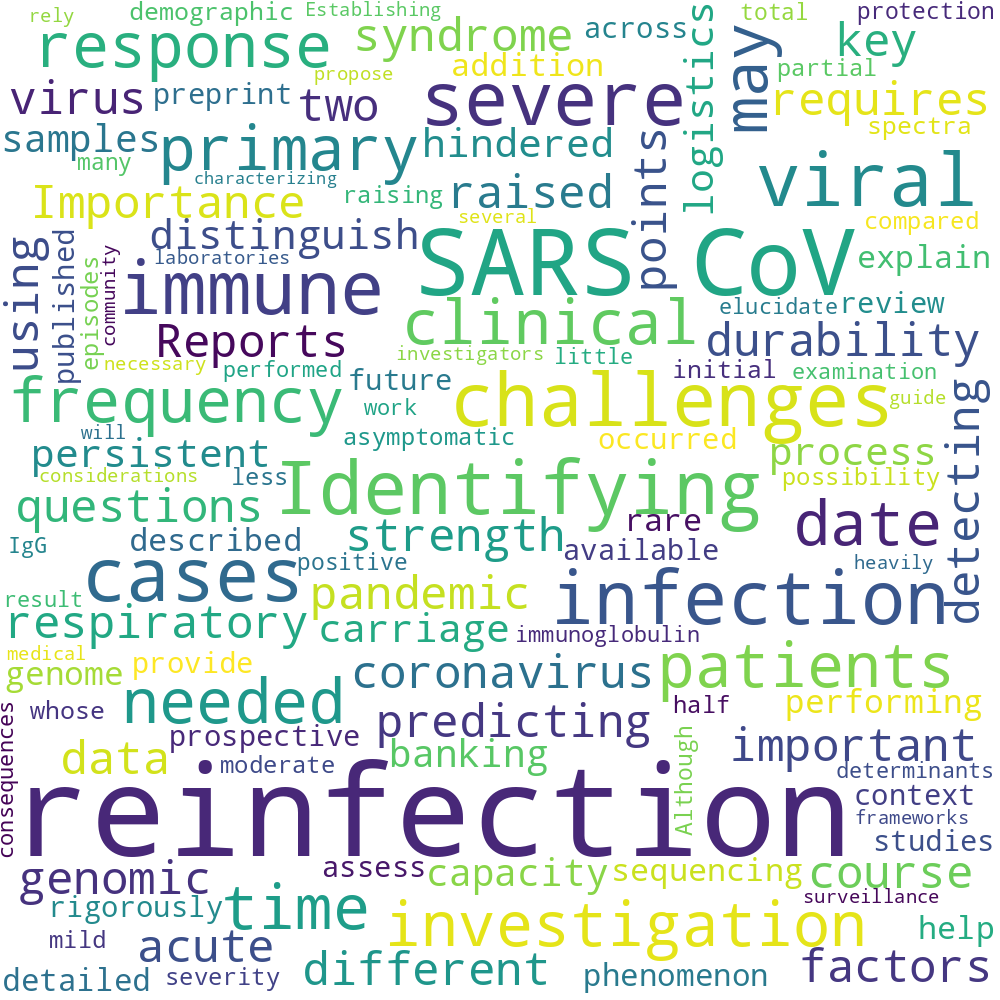
\includegraphics[width=.75\linewidth]{img/severeacuterespiratorysyndromecoronavirus.png}
            \caption{Wordcloud of most frequent terms within section severe acute respiratory syndrome coronavirus.}
            \label{fig:wcl_severeacuterespiratorysyndromecoronavirus}
        \end{figure}

        \begin{table}[H]
        \scriptsize
        \centering
        \caption{Articles adherent to section Severe Acute Respiratory Syndrome Coronavirus}
        \renewcommand{\arraystretch}{1.5}
        \begin{tabular}{p{0.5\textwidth}l}
            \toprule 
            Title & DOI* \\     \midrule The Importance and Challenges of Identifying SARS CoV 2 Reinfections. \cite{TheImport6b3e7387} & \href{https://dx.doi.org/10.1128/JCM.02769 20; }{10.1128/JCM.02769 20; }\\     \midrule
            * Clickable item \\
            \bottomrule
        \end{tabular}
        \label{tab:topic12}
        \end{table}\section{Situ Aortoiliac Reconstruction Cryopreserved Allografts}
            Long term results of cryopreserved allografts in aortoiliac graft infections.OBJECTIVE  Different graft materials have been proposed for in situ reconstruction in the setting of vascular graft infection (VGI). We analyzed the long term outcomes after in situ aortoiliac reconstruction with cryopreserved allografts. METHODS  We performed a retrospective analysis of patients who had undergone in situ aortoiliac reconstruction with cryopreserved arterial allografts for VGI from 2000 to 2015. The end points were the perioperative and long term mortality and graft related complications, including stenosis, occlusion, pseudoaneurysm, and reinfection. RESULTS  A total of 33 patients (91% male) with a median age of 67 years (range, 53 83 years) had undergone in situ aortoiliac reconstruction with cryopreserved allografts. The 30 day mortality was 6% (n = 2); both deaths were related to the allograft (one early allograft enteric fistula and one graft rupture). Another two patients had experienced early (≤30 days) graft related events (one allograft enteric fistula and one graft limb occlusion), for an early graft related complication rate of 12% (n = 4). Of the 31 discharged patients, 13 (42%) had died after a median of 47 months (range, 2 97 months). The median follow up for the 18 remaining patients was 96 months (range, 10 146 months). The estimated survival at 1, 3, and 5 years was 88%, 81%, and 66%, respectively. Nine patients (29%) had experienced at least one of the following graft related events during follow up, including graft stenosis requiring intervention in five (16%), graft occlusion in four (13%), pseudoaneurysm in three (10%), and reinfection in two patients (6%). The estimated freedom from any first graft related event at 1, 3, and 5 years was 78%, 71%, and 62%, respectively. The estimated primary patency and primary assisted patency at 1 and 3 years was 87% and 79%, and 90% and 83%, respectively. CONCLUSIONS  In situ aortoiliac reconstruction with cryopreserved allografts to treat VGI was associated with relevant perioperative graft related complications. Although the reinfection rate was acceptable, other graft related complications were frequent in the long term, in particular, graft occlusion and stenosis.

        \begin{figure}[H]
            \centering
            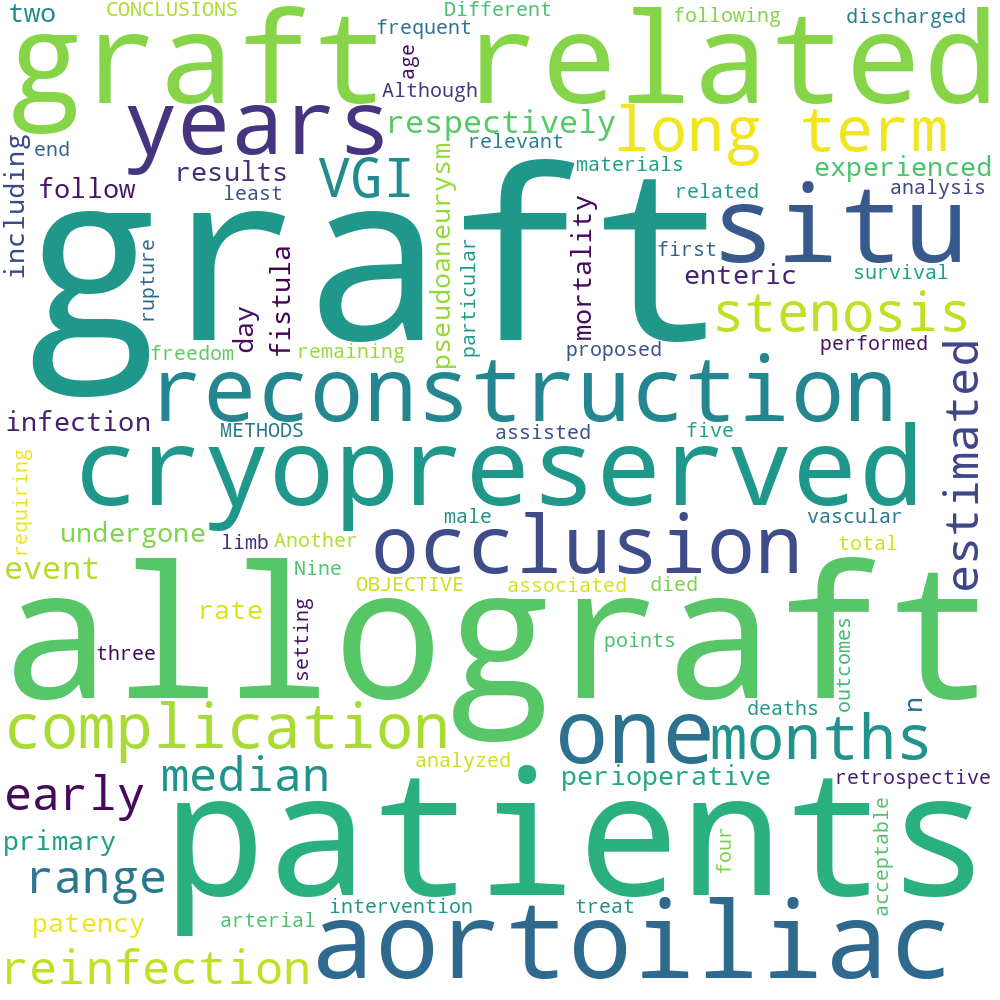
\includegraphics[width=.75\linewidth]{img/situaortoiliacreconstructioncryopreservedallografts.png}
            \caption{Wordcloud of most frequent terms within section situ aortoiliac reconstruction cryopreserved allografts.}
            \label{fig:wcl_situaortoiliacreconstructioncryopreservedallografts}
        \end{figure}

        \begin{table}[H]
        \scriptsize
        \centering
        \caption{Articles adherent to section Situ Aortoiliac Reconstruction Cryopreserved Allografts}
        \renewcommand{\arraystretch}{1.5}
        \begin{tabular}{p{0.5\textwidth}l}
            \toprule 
            Title & DOI* \\     \midrule Long term results of cryopreserved allografts in aortoiliac graft infections. \cite{Longterm77108372} & \href{https://dx.doi.org/; 10.1016/j.jvs.2020.12.070}{; 10.1016/j.jvs.2020.12.070}\\     \midrule
            * Clickable item \\
            \bottomrule
        \end{tabular}
        \label{tab:topic13}
        \end{table}\section{Spontaneous Clearance}
            HCV reinfection rates after cure or spontaneous clearance among HIV infected and uninfected men who have sex with men.BACKGROUND & AIMS  Hepatitis C virus (HCV) reinfection among high risk groups threatens HCV elimination goals. We assessed HCV reinfection rates among men who have sex with men (MSM) in British Columbia (BC), Canada. METHODS  We used data from the BC Hepatitis Testers Cohort, which includes nearly 1.7 million individuals tested for HCV or HIV in BC. MSM who had either achieved sustained virologic response (SVR) after successful HCV treatment, or spontaneous clearance (SC) and had ≥1 subsequent HCV RNA measurement, were followed from the date of SVR or SC until the earliest of reinfection, death, or last HCV RNA measurement. Predictors of reinfection were identified by Cox proportional modelling. The earliest study start date was 6 November 1997 and latest end date was 13 April 2018. RESULTS  Of 1349 HCV positive MSM who met the inclusion criteria, 493 had SC while 856 achieved SVR. 349 (25.65%) had HIV coinfection. We identified 98 reinfections during 5203 person years (PYs) yielding a reinfection rate of 1.88/100PYs. The reinfection rate among SC (2.74/100PYs) was more than twice that of those with SVR (1.03/100 PYs). Problematic alcohol use (aHR 1.73, 95% CI 1.003 2.92), injection drug use (aHR 2.60, 95% CI 1.57 4.29) and HIV coinfection (aHR 2.04, 95% CI 1.29 3.23) were associated with increased risk of HCV reinfection. Mental health counselling history (aHR 0.24, 95% CI 0.13 0.46) was associated with reduced HCV reinfection risk. CONCLUSIONS  There is the need to engage MSM in harm reduction and prevention services following treatment to reduce reinfection risk.

        \begin{figure}[H]
            \centering
            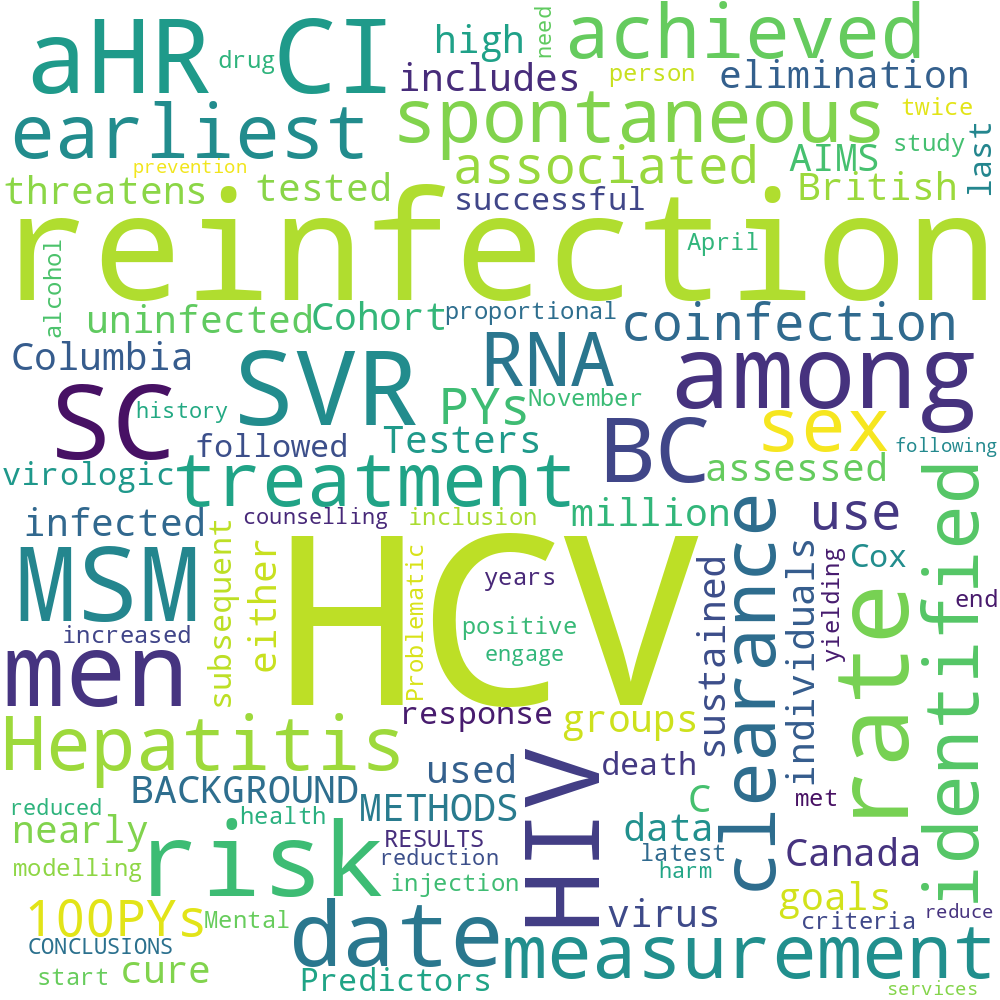
\includegraphics[width=.75\linewidth]{img/spontaneousclearance.png}
            \caption{Wordcloud of most frequent terms within section spontaneous clearance.}
            \label{fig:wcl_spontaneousclearance}
        \end{figure}

        \begin{table}[H]
        \scriptsize
        \centering
        \caption{Articles adherent to section Spontaneous Clearance}
        \renewcommand{\arraystretch}{1.5}
        \begin{tabular}{p{0.5\textwidth}l}
            \toprule 
            Title & DOI* \\     \midrule HCV reinfection rates after cure or spontaneous clearance among HIV infected and uninfected men who have sex with men. \cite{HCVreinfeb27188c6} & \href{https://dx.doi.org/10.1111/liv.14762}{10.1111/liv.14762}\\     \midrule
            * Clickable item \\
            \bottomrule
        \end{tabular}
        \label{tab:topic14}
        \end{table}\section{Susceptibility Infections}
            Homotypic and Heterotypic Protection and Risk of Reinfection Following Natural Norovirus Infection in a Highly Endemic Setting.BACKGROUND  Norovirus is a leading cause of acute gastroenteritis worldwide, yet there is limited information on homotypic or heterotypic protection following natural infection to guide vaccine development. METHODS  A total of 6020 stools collected from 299 Peruvian children between 2010 and 2014 were tested by norovirus real time reverse transcription polymerase chain reaction followed by sequence based genotyping. Cox proportional hazards models were used to derive adjusted hazard ratios (HRs) of infection among children with vs without prior exposure. RESULTS  Norovirus was detected in 1288 (21.3%) samples. GII.4 (26%), GII.6 (19%), and GI.3 (9%) viruses accounted for 54% of infections. Homotypic protection for GI.3 (HR, 0.35; P = .015), GI.7 (HR, 0.19; P = .022), GII.4 (HR, 0.39; P < .001), and GII.6 (HR, 0.52; P = .006) infections was observed. Hazard analysis showed that children with prior GII.4 infection exhibited heterotypic protection with a 48% reduction of subsequent GI.3 infection (HR, 0.52; P = .005). Prior exposure to GI.3, GII.2, and GII.17 infections enhanced susceptibility to subsequent infections with several other norovirus genotypes. CONCLUSIONS  Children up to 2 years of age infected with GII.4 noroviruses demonstrated both homotypic and heterotypic protection to reinfection with other genotypes. These data support the need for ongoing vaccine development efforts with GII.4 as the main component and caution the inclusion of genotypes that may enhance susceptibility to infections.

        \begin{figure}[H]
            \centering
            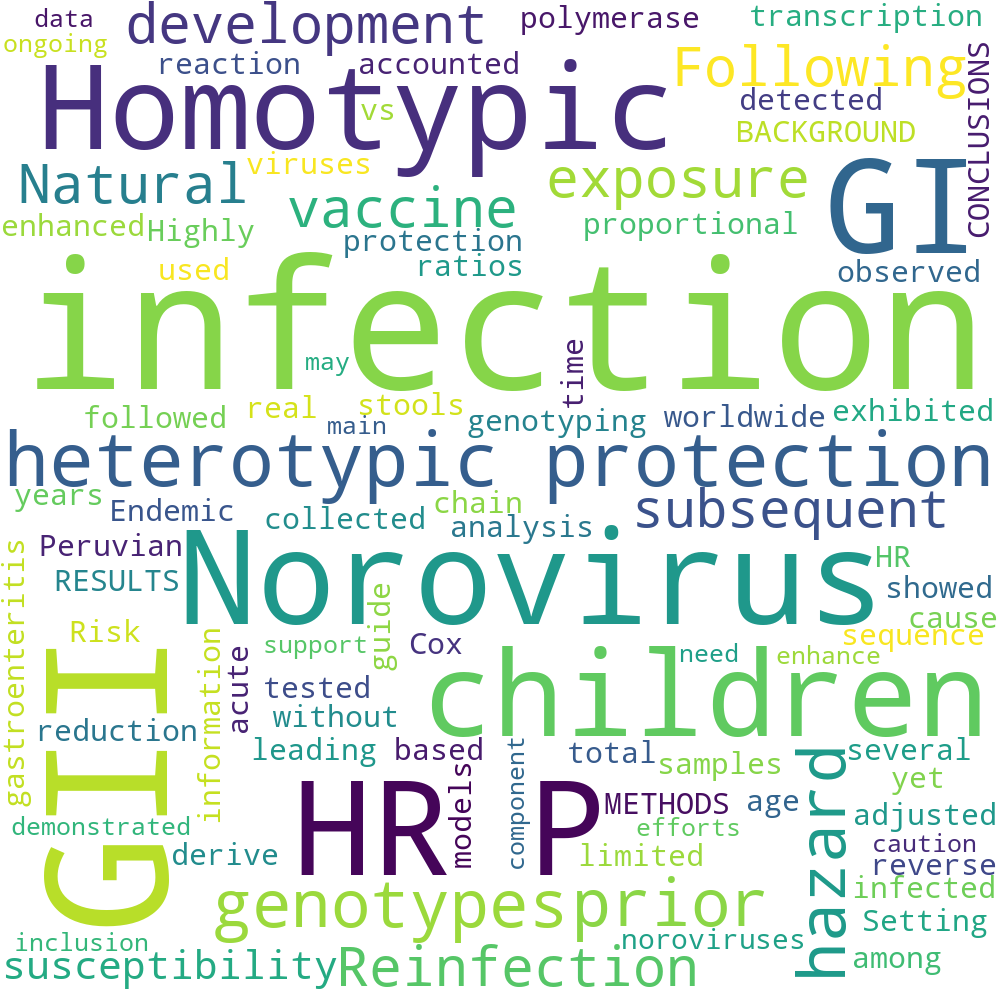
\includegraphics[width=.75\linewidth]{img/susceptibilityinfections.png}
            \caption{Wordcloud of most frequent terms within section susceptibility infections.}
            \label{fig:wcl_susceptibilityinfections}
        \end{figure}

        \begin{table}[H]
            \scriptsize
            \centering
            \caption{Articles adherent to section Susceptibility Infections}
            \renewcommand{\arraystretch}{1.5}
            \begin{tabular}{p{0.5\textwidth}l}
                \toprule 
                Title & DOI* \\     \midrule Homotypic and Heterotypic Protection and Risk of Reinfection Following Natural Norovirus Infection in a Highly Endemic Setting. \cite{Homotypice0418018} & \href{https://dx.doi.org/10.1093/cid/ciaa019}{10.1093/cid/ciaa019}\\     \midrule
                * Clickable item \\
                \bottomrule
            \end{tabular}
            \label{tab:topic15}
        \end{table}
    
    \section{Prospero systematic review}
    \subsection{* Review title}
    Give the working title of the review, for example the one used for obtaining funding. Ideally the title should state succinctly
    the interventions or exposures being reviewed and the associated health or social problems. Where appropriate, the title
    should use the PI(E)COS structure to contain information on the Participants, Intervention (or Exposure) and Comparison
    groups, the Outcomes to be measured and Study designs to be included.
    Acronyms may be included in titles, but should not be used alone without expansion unless they are regarded as more
    usual than the expansion (e.g. HIV).
    The title in this field must be in English. If the original title is in a different language the English version must be entered
    here, with the non-English version entered into the field labeled “Original Language Title”.
    If the final title of the review differs, this can be displayed in the Publication of Final Report Field.
    Example: Systematic review and meta-analysis of recurrence and survival following pre- versus post-operative radiation
    in localized, resectable soft-tissue sarcoma.

    \subsection{Original language title}
    For reviews in languages other than English, this field should be used to enter the title in the language of the review. This
    will be displayed together with the English language title.
    Example: Revisión sistemática y meta-análisis de la recurrencia y la supervivencia tras la fase de radiación en
    comparación con post-operatorio en el sarcoma localizados resecables de tejido blando.

    \subsection{* Anticipated or actual start date}
    Give the date when the systematic review commenced, or is expected to commence.
    For the purposes of PROSPERO, the date of commencement for the systematic review can be defined as any point after
    completion of a protocol but before formal screening of the identified studies against the eligibility criteria begins.
    A protocol can be deemed complete when it is approved by a funder or the person commissioning the review; when peer
    review is complete; when the protocol is published or when the authors decide that it is complete and they do not
    anticipate any major revisions to the design of the systematic review.
    This field may be edited at any time. All edits to published records will appear in the record audit trail. A brief explanation of
    the reason for changes should be given in the Revision Notes facility.

    \textbf{Example}: 01 June 2011.

    \subsection{* Anticipated completion date}
    Give the date by which the review is expected to be completed. In the absence of an agreed contractual date, a realistic
    anticipated date for completion should be set. It can be modified should the schedule change. When this date is reached,
    the named contact will receive an automated email to ask them to provide an update on progress.
    This field may be edited at any time. All edits will appear in the record audit trail. A brief explanation of the reason for
    changes should be given in the Revision Notes facility.

    \textbf{Example}: 01 June 2011.

    \subsection{* Stage of review at time of this submission}
    Indicate the stage of progress of the review by ticking the relevant Started and Completed boxes. Additional information
    may be added in the free text box provided.
    Please note: Reviews that have progressed beyond the point of completing data extraction at the time of initial registration
    are not eligible for inclusion in PROSPERO. Should evidence of incorrect status and/or completion date being supplied at
    the time of submission come to light, the content of the PROSPERO record will be removed leaving only the title and
    named contact details and a statement that inaccuracies in the stage of the review date had been identified.
    This field should be updated when any amendments are made to a published record and on completion and publication of
    the review. If this field was pre-populated from the initial screening questions then you are not able to edit it until the record
    is published.
    The review has not yet started: Yes

    \begin{table}[H]
        \begin{tabular}{lll}
            \textbf{Review stage} & \textbf{Started} & \textbf{Completed} \
            Preliminary searches & No & No \
            Piloting of the study selection process & No & No \
            Formal screening of search results against eligibility criteria & No & No  \
            Data extraction & No & No \
            Risk of bias (quality) assessment & No & No \
            Data analysis & No & No
        \end{tabular}
    \end{table}

    \subsection{* Named contact}

    The named contact acts as the guarantor for the accuracy of the information presented in the register record. This should
    be the lead reviewer or a representative of the review team. This person is also responsible for submitting details of any
    amendments while the review is ongoing and publication details after the review is completed. The named contact is the
    person to whom users of PROSPERO would send questions or comments.

    This field is automatically populated from the named contact’s signing in details. The named contact’s name will be
    displayed in the public record.

    \textbf{Example}: Dr Joseph Bloggs
    N.B. To change the named contact for a published record, send details of the existing and new contact to crdregister@york.ac.uk

    Email salutation (e.g. "Dr Smith" or "Joanne") for correspondence:


    \subsection{* Named contact email}
    Give the electronic mail address of the named contact. This may be a generic email address to which the named contact
    has access.

    This field is automatically populated from the named contact’s joining details, but can be changed if required. The email
    address supplied here will be displayed in the public record.

    \textbf{Examples:} joseph.bloggs@city.ac.uk or research.secretary@city.ac.uk

    \subsection{Named contact address}
    PLEASE NOTE this information will be published in the PROSPERO record so please do not enter private information

    Give the full postal address for the named contact. (N.B. This field is automatically populated from the named contact’s
    joining details.)
    This address will be displayed in the public record. If you do not wish it to appear in the public record delete the content of
    this field.

    \textbf{Example:} Alcuin B Block,University of York, York, YO10 5DD, UK

    \subsection{Named contact phone number}
    Give the telephone number for the named contact, including international dialling code.
    (N.B. This field is automatically populated from the named contact’s joining details.)

    This number will be displayed in the public record. If you do not wish it to appear in the public record delete the content of
    this field.

    \textbf{Example:} +44 (0)10904 321040

    \subsection{* Organisational affiliation of the review}
    Full title of the organisational affiliations for this review and website address if available. This field may be completed as
    ‘None’ if the review is not affiliated to any organisation

    \textbf{Example:} Andalusian Agency for Health Technology Assessment (AETSA)

    \textbf{Organisation web address:}

    \subsection{* Review team members and their organisational affiliations}
    Give the personal details and the organisational affiliations of each member of the review team. Affiliation refers to groups
    or organisations to which review team members belong. \textbf{NOTE: email and country are now mandatory fields for each
    person..} Affiliation refers to groups or organisations to which review team members belong.

    Review team members will be listed ‘manuscript’ style in the order entered in this list. The named contact will be
    automatically added to this field, but can be deleted if not a member of the review team. To place the named contact
    somewhere other than first in order, delete the automatic entry and enter members’ details in the required order.

    Membership of the review team and details of affiliations can be updated at any time.
    All edits will appear in the record audit trail.

    \textbf{Example:} Mr Joseph Bloggs, Centre for Reviews and Dissemination, University of York, UK. Dr Jane Smith, Department
    of Health Sciences, University of York, UK. Prof. Steven Jones, Centre for Health Statistics, Medical Research Centre,
    Canada.

    \subsection{* Funding sources/sponsors}
    Give details of the individuals, organizations, groups or other legal entities who take responsibility for initiating, managing,
    sponsoring and/or financing the review. Include any unique identification numbers assigned to the review by the individuals
    or bodies listed.

    \textbf{Examples:} NIHR HTA Programme (Project ref 09/13/02). The Terry Fox New Frontiers Program in Cancer (Ref
    201006TFL). Funding provided by Amgen, Merck, Roche, and Sanofi-aventis.

    \textbf{Grant number(s)}

    \subsection{* Conflicts of interest}
    List any conditions that could lead to actual or perceived undue influence on judgements concerning the main topic
    investigated in the review. The conflicts of interest listed should cover the review team as a whole, as well as individuals in
    the team.

    Conflicts of interest arise when a team member or the team as a whole (e.g. because of the team’s institution) has financial
    or personal relationships that may inappropriately influence (bias) their actions (such relationships are also known as dual
    commitments, competing interests, or competing loyalties).These relationships vary from being negligible to having great
    potential for influencing judgment. Not all relationships represent true conflict of interest.

    On the other hand, the potential for conflict of interest can exist regardless of whether a person believes that the
    relationship affects his or her scientific judgment. Financial relationships (such as employment, consultancies, stock
    ownership, honoraria, and paid expert testimony) are the most easily identifiable conflicts of interest and the most likely to
    undermine the credibility of the review.

    However, conflicts can occur for other reasons, such as personal relationships, academic competition, and intellectual
    passion. For the purposes of disclosure, the term “competing interest” should be considered synonymous with conflict of
    interest.

    \textbf{Example:} The lead reviewer (JB) has given talks on this topic at workshops, seminars, and conferences for which travel
    and accommodation has been paid for by the organisers. The other authors declare that they have no known conflicts of
    interest.

    \textbf{None}

    \subsection{Collaborators}
    Give the name and affiliation of any individuals or organisations who are working on the review but who are not listed as
    review team members. NOTE: email and country are now mandatory fields for each person.

    \textbf{Example:} Dr Eric Porter, Oncologist, University Hospital, Brighton, UK. Clinical advisor.


    \subsection{* Review question}
    State the question(s) to be addressed by the review, clearly and precisely. Review questions may be specific or broad. It
    may be appropriate to break very broad questions down into a series of related more specific questions. Questions may be
    framed or refined using PI(E)COS where relevant.

    \textbf{Example:} How does pre-operative chemotherapy impact on survival of early stage non-small cell lung cancer compared
    to surgery alone?

    \subsection{* Searches}
    State the sources that will be searched. Give the search dates, and any restrictions (e.g. language or publication period).
    Do NOT enter the full search strategy (it may be provided as a link or attachment.)
    The search strategy reported in systematic review protocols should:
    \begin{itemize}
        \item Name all sources that will be used to identify studies for the systematic review.
    \end{itemize}
    Sources include (but are not limited to) bibliographic databases, reference lists of eligible studies and review articles, key
    journals, conference proceedings, trials registers, Internet resources and contact with study investigators, experts and
    manufacturers.

    Systematic reviews typically use more than one database. Examples of electronic bibliographic databases include
    MEDLINE, EMBASE, PsycINFO. Other database sources include The Cochrane Library, Health Technology Assessment
    Database, and Web of Science.
    \begin{itemize}
        \item Search dates (from and to)
        \item Restrictions on the search including language and publication period
        \item Whether searches will be re-run prior to the final analysis
    \end{itemize}

    It is considered good practice for searches to be re-run just before the final analyses and any further studies identified,
    retrieved for inclusion. 
    \begin{itemize}
        \item Whether unpublished studies will be sought
    \end{itemize}

    \subsection{URL to search strategy}
    Give a link to the search strategy or an example of a search strategy for a specific database if available (including the
    keywords that will be used in the search strategies).
    Alternatively, an electronic file could be supplied which will be linked to from the Register record. This will be made publicly
    available from the published record immediately, or it can be held in confidence until the review has been completed, at
    which time it will be made publicly available.

    \textbf{Example}: http://www.biomedcentral.com/1756-0500/3/250

    Do not make this file publicly available until the review is complete

    \subsection{* Condition or domain being studied}
    Give a short description of the disease, condition or healthcare domain being studied. This could include health and
    wellbeing outcomes.
    \textbf{Examples}: Type 2 diabetes. Physical activity in children.

    \subsection{* Participants/population}
    Give summary criteria for the participants or populations being studied by the review. The preferred format includes details
    of both inclusion and exclusion criteria.

    \textbf{Example}:
    Inclusion: Adults with schizophrenia (as diagnosed using any recognised diagnostic criteria).
    Exclusion: Adolescents (under 18 years of age) and elderly people (over 70).

    \subsection{* Intervention(s), exposure(s)}
    Give full and clear descriptions or definitions of the nature of the interventions or the exposures to be reviewed. This is
    particularly important for reviews of complex interventions (interventions involving the interaction of several elements). If
    appropriate, an operational definition describing the content and delivery of the intervention should be given.

    Ideally, an intervention should be reported in enough detail that others could reproduce it or assess its applicability to their
    own setting. The preferred format includes details of both inclusion and exclusion criteria.

    For reviews of qualitative studies give details of the focus of the review.

    \textbf{Example}: Population-level tobacco control interventions are defined as those applied to populations, groups, areas,
    jurisdictions or institutions with the aim of changing the social, physical, economic or legislative environment to make them
    less conducive to smoking. These are approaches that mainly rely on state or institutional control, either of a link in the
    supply chain or of smokers' behaviour in the presence of others.

    Examples include tobacco crop substitution or diversification, removing subsidies on tobacco production, restricting trade
    in tobacco products, measures to prevent smuggling, measures to reduce illicit cross-border shopping, restricting
    advertising of tobacco products, restrictions on selling tobacco products to minors, mandatory health warning labels on
    tobacco products, increasing the price of tobacco products, restricting access to cigarette vending machines, restricting
    smoking in the workplace, and restricting smoking in public places. Such approaches could also form part of wider,
    multifaceted interventions in schools, workplaces or communities.

    \subsection{* Comparator(s)/control}
    Where relevant, give details of the alternatives against which the main subject/topic of the review will be compared (e.g.
    another intervention or a non-exposed control group). The preferred format includes details of both inclusion and exclusion
    criteria.

    Control or comparison interventions should be described in as much detail as the intervention being reviewed. If the
    comparator is ‘treatment as usual’ or ‘standard care’, this should be described, with attention being paid to whether it is
    ‘standard care’ at the time that an eligible study was done, or at the time the review is done.

    Systematic reviews of qualitative studies rarely have a comparator or control; stating ‘Not applicable’ is therefore
    acceptable.

    \textbf{Examples}: Placebo. A group of hospital in-patients who were not exposed to the infectious agent.


    \subsection{* Types of study to be included}
    Give details of the types of study (study designs) eligible for inclusion in the review. If there are no restrictions on the types
    of study design eligible for inclusion, or certain study types are excluded, this should be stated. The preferred format
    includes details of both inclusion and exclusion criteria.

    If different study designs are needed for different parts of the review, this should be made clear. Where qualitative
    evidence will be incorporated in or alongside a review of quantitative data, this should be stated.

    \textbf{Example}: We will include randomised trials to assess the beneficial effects of the treatments, and will supplement these
    with observational studies (including cohort and case–control studies) for the assessment of harms.

    \subsection{Context}

    \subsection{* Main outcome(s)}

    \subsection{* Additional outcome(s)}

    \subsection{* Data extraction (selection and coding)}

    \subsection{* Risk of bias (quality) assessment}

    \subsection{* Strategy for data synthesis}

    \subsection{* Analysis of subgroups or subsets}

    \subsection{* Type and method of review}

    \subsection{Language}

    \subsection{* Country}

    \subsection{Other registration details}

    \subsection{Reference and/or URL for published protocol}

    \subsection{Dissemination plans}

    \subsection{Keywords}

    \subsection{Details of any existing review of the same topic by the same authors}

    \subsection{Current review status}

    \subsection{Any additional information}

    \subsection{Details of final report/publication(s)}
        

    \bibliographystyle{abbrv}
\end{document}
